% 15.01.2015

\section{Determinanten}

\label{Determinanten}

\subsection{Grundlagen}

\subsubsection{Geometrische Motivation}

Sei $ n \in \N $ und $ a_1, \ldots, a_n \in \R^n $. Sei $ P(a_1, \ldots, a_n) := \{ \sum_{i=1}^n \alpha_ia_i : \alpha_1, \ldots, \alpha_n \in [0,1] \} $. Wenn $ a_1, \ldots, a_n $ linear unabhängig sind, dann heißt $ P(a_1, \ldots, a_n) $ \emph{Parallelotop} (\emph{Parallelepiped} im Fall $ n=3 $, \emph{Parallelogramm} im Fall $ n=2 $). Sei $ V(a_1, \ldots, a_n) $ das \emph{Volumen} von $ P(a_1, \ldots, a_n) $ (Flächeninhalt im Fall $ n=2 $). Volumen wird in der Analysis eingeführt.
\begin{itemize}
	\item
		$ V(a_1, \ldots, a_n) $ ist \glqq zum Teil linear\grqq\ in den Vektorargumenten $ a_1, \ldots, a_n $. $ V(a_1, a'_2 + a''_2) = V(a_1,a'_2) + V(a_1,a''_2) $, wenn $ a'_2 $ und $ a''_2 $ auf derselben Seite von $ \lin(a_1) $ liegen (siehe Bild).
	\item
		$ V(\lambda a_1, a_2) = \lambda V(a_1, a_2) $, falls $ \lambda \geq 0 $ (siehe Bild).
	\item
		Betrachten wir den Fall $ a_1 = (l,0), a_2 = (s,h) $ mit $ l,s,h \in \R $. $ V(a_1,a_2) = |lh| $.
\end{itemize}
Es stellt sich heraus, dass $ \pm V(a_1, \ldots, a_n) $ mit einem Vorzeichen, das von der Orientierung des Systems $ a_1, \ldots, a_n $ abhängig ist, linear in jedem der $ n $ Vektoren $ a_1, \ldots, a_n $ ist.

%TODO: mit subfigures aufhübschen: Orientierungen für n=2 und n=3

\subsubsection{Definierende Eigenschaften}

\begin{thm}
	Sei $ n \in \N $. Es existiert genau eine Funktion $ \det : \overbrace{\K^n \times \ldots \times \K^n}^\text{$ n $ mal} \to \K $ mit den folgenden Eigenschaften:
	\begin{itemize}
		\item[\normalfont(D1)]
			$ \det $ ist linear in jedem der $ n $ Vektorargumente, d.h.:
			
			$ \det(a_1, \ldots, a_{i-1}, \alpha u + \beta v, \alpha_{i+1}, \ldots, a_n) =
			\begin{aligned}[t]
				&\: \alpha\det(a_1, \ldots, a_{i-1}, u, \alpha_{i+1}, \ldots, a_n) \\
				+ &\: \beta\det(a_1, \ldots, a_{i-1}, v, \alpha_{i+1}, \ldots, a_n)
			\end{aligned} $
			
			für alle $ a_1, \ldots, a_n, u, v \in \K^n $, $ \alpha, \beta \in \K $ und $ i \in \is{1}{n} $.
		\item[\normalfont(D2)]
			$ \det $ ist alternierend, d.h. wenn $ a_i = a_j $ für zwei Indizes $ i,j \in \is{1}{n} $ mit $ i \neq j $, dann $ \det(a_1, \ldots, a_n) = 0 $ für alle $ a_1, \ldots, a_n \in \K^n $.
		\item[\normalfont(D3)]
			$ \det(e_1, \ldots, e_n) = 1 $.
	\end{itemize}
\end{thm}

\noindent Der Beweis wird später gegeben. Zunächst wird $ \det $ als eine beliebige Funktion mit (D1), (D2), (D3) behandelt (ohne zu verifizieren, ob eine solche Funktion existiert oder eindeutig ist).

Sei $ n \in \N $ und sei $ A = (a_{ij})_{i,j=1}^n = (a_1|\ldots|a_n) \in \K^{n \times n} $. Wir nennen $ \det(A) := \det(a_1, \ldots, a_n) $ die \emph{Determinante} von $ A $. Eine weitere Bezeichnung:
\begin{equation}
	\left| \begin{matrix}
		a_{11} & \cdots & a_{1n} \\
		\vdots & \ddots & \vdots \\
		a_{n1} & \cdots & a_{nn}
	\end{matrix} \right|
\end{equation}

\subsubsection{Weitere Eigenschaften}

\begin{thm}
	Sei $ n \in \N $. Sei $ A = (a_{ij}) \in \K^{n \times n} $. Dann gilt:
	\begin{itemize}
		\item[\normalfont(D4)]
			$ \det(\lambda A) = \lambda^n \det(A) $ für alle $ \lambda \in \K $.
		\item[\normalfont(D5)]
			Enthält $ A $ eine Nullspalte, dann gilt $ \det(A) = 0 $.
		\item[\normalfont(D6)]
			Entsteht $ B $ durch Vertauschung von zwei Spalten von $ A $, dann gilt $ \det(B) = -\det(A) $.
			
			Mit anderen Worten ändern die Elementartransformationen von Spalten vom Typ 1 das Vorzeichen der Determinante, da sich die Orientierung der Vektoren ändert.
		\item[\normalfont(D7)]
			Entsteht $ B $ aus $ A $ durch Addition der $ \lambda $-fachen $ j $-ten Spalte zur $ i $-ten Spalte (mit $ \lambda \in \K $, $ i,j \in \is{1}{n} $ und $ i \neq j $), so gilt $ \det(B) = \det(A) $.
			
			Mit anderen Worten ändern die Elementartransformationen von Spalten vom Typ 3 die Determinante nicht.
		\item[\normalfont(D8)]
			Ist $ A $ eine obere Dreiecksmatrix, so gilt $ \det(A) = a_{11} \cdot \ldots \cdot a_{nn} $.
		\item[\normalfont(D9)]
			Ist $ n \geq 2 $ und hat $ A $ die Form $ A = \begin{pmatrix} B & C \\ O & D \end{pmatrix} $ mit $ B \in \K^{k \times k} $, $ C \in \K^{k \times (n-k)} $ und $ D \in \K^{(n-k) \times (n-k)} $ und $ k \in \is{1}{n-1} $, dann gilt $ \det(A) = \det(B)\det(D) $.
		\item[\normalfont(D10)]
			$ \det(A) = 0 \Leftrightarrow \rang(A) < n $.
		\item[\normalfont(D11)]
			Für jede $ B \in \K^{n \times b} $ gilt $ \det(AB) = \det(A)\det(B) $. Insbesondere, wenn $ A $ invertierbar ist, dann gilt $ \det(A) \neq 0 $ und $ \det(A^{-1}) = \det(A)^{-1} $.
	\end{itemize}
\end{thm}
\begin{proof}\
	\begin{itemize}
		\item[\normalfont(D4)]
			folgt aus (D1):
			
			$ \det(\lambda A) = \det(\lambda a_1, \ldots, \lambda a_n) = \lambda^n \det(a_1, \ldots, a_n) = \lambda^n \det(A) $.
		\item[\normalfont(D5)]
			Der Einfachheit halber sei $ a_1 = 0 $. Dann gilt:
			
			$ \det(A) = \det(0, a_2, \ldots, a_n) = \det(0 \cdot 0, a_2, \ldots, a_n) = 0 \cdot \det(0, a_2, \ldots, a_n) = 0 $.
		\item[\normalfont(D6)]
			Der Einfachheit halber wird angenommen, dass $ B $ durch Vertauschen der ersten und zweiten Spalte von $ A $ entsteht.
			
			$ \begin{aligned}
				0 &= \det(a_1 + a_2, a_1 + a_2, a_3, \ldots, a_n) \\
				&= \det(a_1, a_1 + a_2, a_3, \ldots, a_n) + \det(a_2, a_1 + a_2, a_3, \ldots, a_n) \\
				&= \det(a_1, a_1, a_3, \ldots, a_n) + \det(a_1, a_2, a_3, \ldots, a_n) \\
				&\quad + \det(a_2, a_1, a_3, \ldots, a_n) + \det(a_2, a_2, a_3, \ldots, a_n) \\
				&= 0 + \det(A) + \det(B) + 0 \\
				\Rightarrow \det(B) &= -\det(A). 
			\end{aligned} $
		\item[\normalfont(D7)]
			O.B.d.A. sei $ i=1 $ und $ j=2 $. \hfill 21.01.2015
			
			$ \begin{aligned}
				\det(B) &= \det(a_1 + \lambda a_2, a_2, \ldots, a_n) \\
				&= \det(a_1, a_2, \ldots, a_n) + \lambda\det(a_2, a_2, \ldots, a_n) \\
				&= \det(a_1, a_2, \ldots, a_n) + \lambda \cdot 0 \\
				&= \det(A).
			\end{aligned} $
		\item[\normalfont(D8)]
			Sei $ A =
			\begin{pmatrix}
				a_{11} & \cdots & a_{1n} \\
				& \ddots & \vdots \\
				& & a_{nn}
			\end{pmatrix} $ eine obere Dreiecksmatrix.
			
			Wir betrachten den Fall, dass $ a_{ii} = 0 $ ist, für ein $ i \in \is{1}{n} $. Wir fixieren das kleinstmögliche $ i $ wie oben, d.h. $ a_{jj} \neq 0 \: \forall i \in \is{1}{n} $ mit $ j < i $.
			
			Wir verwenden eine Spaltentransformation, um mit Hilfe der $ (i-1) $-ten Spalte die $ (i-1) $-te Komponente der $ i $-ten Spalte durch 0 zu ersetzen. Wir verwenden anschließend eine Spaltentransformation vom Typ 3, um mit Hilfe der $ (i-2) $-ten Spalte die $ (i-2) $-te Komponente der $ i $-ten Spalte durch 0 zu ersetzen. Die iterative Fortsetzung dieser Prozedur erzeugt eine Matrix, deren $ i $-te Spalte eine 0-Spalte ist.
			
			Eine Matrix mit einer 0-Spalte hat die Determinante 0. Da die Spaltentransformationen vom Typ 3 die Determinante nicht ändern, folgt $ \det(A) = 0 $.
			
			Wir betrachten nun den Fall, dass $ a_{ii} \neq 0 \: \forall i \in \is{1}{n} $. Mit Hilfe von Spaltentransformationen vom Typ 3 ersetzt man die zweite Komponente der Spalten 3 bis $ n $ durch 0, usw.
			
			Mit dieser Prozedur wird $ A $ zur Diagonalmatrix konvertiert. D.h. es gilt:
			
			$ \begin{aligned}
				\det(A) &= \det\begin{pmatrix}
					a_{11} && \\
					& \ddots & \\
					&& a_{nn}
				\end{pmatrix} \\
				&= \det(a_{11}e_1, \ldots, a_{nn}e_n) \\
				&= a_{11} \cdots a_{nn} \cdot \det(e_1, \ldots, e_n) \\
				&= a_{11} \cdots a_{nn}.
			\end{aligned} $
		\item[\normalfont(D9)]
			Sei $ A =
			\begin{pmatrix}
				B & C \\
				O & D
			\end{pmatrix} $
			mit $ B \in \K^{k \times k}, D \in \K^{(n-k) \times (n-k)} $ und $ k \in \is{1}{n} $.
			
			Die Matrizen $ B $ und $ D $ lassen sich durch Spaltentransformationen vom Typ 1 (Vertauschung) und Typ 3 zu oberen Dreiecksmatrizen $ B' $ und $ D' $ konvertieren. (Im Wesentlichen verwendet man dabei das Gaußverfahren.)
			
			Den Spaltentransformationen, die man bei der Konvertierung von $ B $ zu $ B' $ und $ D $ zu $ D' $ benutzte, kann man Spaltentransformationen der Matrix $ A $ zuordnen, welche die Matrix $ A $ zu einer Matrix der Form $ A' =
			\begin{pmatrix}
				B' & C' \\
				O & D'
			\end{pmatrix} $
			überführen.
			
			Die Matrizen $ A', B' $ und $ D' $ sind diagonal:
			
			$ \det(A') = \det(B')\det(D') $
			
			Sei $ s $ die Anzahl der Transformationen vom Typ 1, die bei der Konvertierung von $ B $ benutzt wurden. Sei $ t $ die Anzahl der Transformationen vom Typ 1, die bei der Konvertierung von $ D $ benutzt wurden.
			
			Dann ist $ s+t $ die Anzahl der Transformationen vom Typ 1, die bei der Konvertierung von $ A $ benutzt wurden. Es gilt:
			
			$ \begin{aligned}
				\det(A') &= (-1)^{s+t} \det(A) \\
				\det(B') &= (-1)^s \det(B) \\
				\det(D') &= (-1)^t \det(D)
			\end{aligned} $
			
			Die vorigen Gleichungen und $ (\ast) $ ergeben $ \det(A) = \det(B)\det(D) $.
		\item[\normalfont(D10)]
			Im Fall $ n=1 $ ist die Behauptung trivial. Sei $ n \geq 2 $. Im Fall $ \rang(A) < n $ ist eine der Spalten von $ A $ Linearkombination der restlichen Spalten. O.B.d.A. sei $ a_1 = \sum_{i=2}^n \lambda_i a_i $ mit $ \lambda_2, \ldots, \lambda_n \in \K $.
			
			$ \begin{aligned}
				\det(A) &= \det(a_1, \ldots, a_n) \\
				&= \det\left(\sum_{i=2}^n \lambda_i a_i, a_2, \ldots, a_n\right) \\
				&= \sum_{i=2}^n \lambda_i \det(a_i, a_2, \ldots, a_n) \\
				&= \sum_{i=2}^n \lambda_i \cdot 0 = 0
			\end{aligned} $
			
			Im Fall $ \rang(A) = n $ zeigen wir, dass $ \det(A) \neq 0 $ ist. Wir konvertieren $ A $ zu einer oberen Dreiecksmatrix mit der Verwendung von Spaltentransformationen vom Typ 1 und 3. Dafür wird im Wesentlichen das Gaußverfahren benutzt.
			
			$ A = \begin{pmatrix}
				| && | \\
				a_1 & \cdots & a_n \\
				| && |
			\end{pmatrix}
			= \begin{pmatrix}
				a_{11} & \cdots & a_{1n} \\
				\vdots & \ddots & \vdots \\
				a_{n1} & \cdots & a_{nn}
			\end{pmatrix} $
			
			Die $ n $-te Komponente einer der Spalten $ a_1, \ldots, a_n $ ist ungleich Null, denn sonst wäre $ \rang(A) < n $.
			
			Durch die Verwendung von Spaltentransformationen vom Typ 1 kann man annehmen, dass $ a_{m,n} \neq 0 $ ist. Mit Transformationen vom Typ 3 kann man anschließend die Komponenten $ a_{n,1}, \ldots, a_{n,n-1} $ durch 0 ersetzen.
			
			$ A' = \begin{pmatrix}
				&&\tikz[na] \node[coordinate] (n1) {};& \ast \\
				& B && \vdots \\
				\tikz[na] \node[coordinate] (n3) {};&&\tikz[na] \node[coordinate] (n2) {};& \ast \\
				0 & \cdots & 0 & a_{nn}
			\end{pmatrix}
			\text{, wobei $ B \in \K^{(n-1) \times (n-1)} $ und $ a_{nn} \neq 0 $.} $
			\begin{tikzpicture}[overlay]
				\draw (n1) -- (n2) -- (n3);
			\end{tikzpicture}
			
			Nach dieser Modifizierung von $ A $ ist der Rang der Matrix $ (a_{ij})_{i,j=1}^{n-1} \in \K^{(n-1) \times (n-1)} $ gleich $ n-1 $.  Denn sonst wären die $ n-1 $ Spalten dieser Matrix und somit auch die ersten $ n-1 $ Spalten von $ A $ linear abhängig, was der Bedingung $ \rang(A) = n $ widerspräche.
			
			Durch die iterative Fortsetzung der vorigen Schritte wird $ A $ zu einer oberen Dreiecksmatrix konvertiert, deren Diagonalelemente alle ungleich Null sind. Es folgt $ \det(A) \neq 0 $.
		\item[\normalfont(D11)]
			Im Fall $ \rang(B) < n $ gilt $ \rang(AB) \leq \rang(B) < n $. Somit gilt $ \det(AB) = 0 = \det(A) \cdot 0 = \det(A)\det(B) $.
			
			Im Fall $ \rang(B) = n $ ist $ B $ invertierbar. Die Matrix $ B $ lässt sich durch Spaltentransformationen vom Typ 1,2,3 zur Einheitsmatrix $ I_n $ konvertieren.
			
			Jede Elementartransformation der Spalten kann als Matrixmultiplikation dargestellt werden. Sei $ C = (c_1, \ldots, c_n) \in \K^{n \times n} $ beliebig.
			
			\hfill 22.01.2015
		
			\begin{description}[font=\normalfont]
				\item[Typ 1:]
					Das Vertauschen der $ i $-ten und $ j $-ten Spalte von $ C $ mit $ i,j \in \is{1}{n}, i \neq j $. Diese Transformation kann als $ C \mapsto C \cdot S $ beschreiben werden, wobei $ S $ aus der Einheitsmatrix entsteht, indem man die Elemente in den Positionen $ (i,i) $ und $ (j,j) $ durch Nullen und die Elemente in den Position $ (i,j) $ und $ (j,i) $ durch Einsen ersetzt.
		
					Für die Determinanten gilt:
					\begin{align*}
						\det(CS) &= -\det(C) \\
						\det(S) &= -1
					\end{align*}
				\item[Typ 2:]
					Die $ i $-te Spalte von $ C = (c_1, \ldots, c_n) $ wird durch $ \lambda c_i $ ersetzt, mit $ \lambda \in \K \setminus \{0\} $. Diese Transformation wird als $ C \mapsto C \cdot S $ beschrieben, wobei $ S $ aus der Einheitsmatrix entsteht, indem man das Element in der Position $ (i,i) $ durch $ \lambda $ ersetzt.
					
					Für die Determinanten gilt:
					\begin{align*}
						\det(CS) &= \lambda\det(C) \\
						\det(S) &= \lambda
					\end{align*}
				\item[Typ 3:]
					$ i,j \in \is{1}{n}, i \neq j $. $ C = (c_1, \ldots, c_n) $. Die $ i $-te Spalte wird durch $ c_i + \lambda c_j $ ersetzt, mit $ \lambda \in \K $. Diese Transformation wird als $ C \mapsto CS $ beschrieben, wobei $ S $ aus der Einheitsmatrix entsteht, indem das Element in der Position $ (j,i) $ durch $ \lambda $ ersetzt.
					
					Für die Determinanten gilt:
					\begin{align*}
						\det(CS) &= \det(C) \\
						\det(S) &= \det(e_1, \ldots, e_{i-1}, e_i+\lambda e_j, e_{i+1}, \ldots, e_n) \\
						&= \det(e_1, \ldots, e_n) + \lambda\det(e_1, \ldots, e_{i-1}, e_j, e_{i+1}, \ldots, e_n) \\
						&= 1 + \lambda \cdot 0 = 1
					\end{align*}
			\end{description}
			Da $ \rang(B) = n $, existieren Matrizen $ S_1, \ldots, S_t \in \K^{n \times n} $ ($ t \in \N_0 $), die den Spaltentransformationen vom Typ 1, 2, 3 entsprechen und für die $ B = S_1 \cdot \ldots \cdot S_t $ gilt. Es folgt:
			\begin{align*}
				\det(AB) &= \det(A S_1 \cdots S_t) \\
				&= \det(A S_1 \cdots S_{t-1})\det(S_t) \\
				&\enspace\vdots \\
				&= \det(A)\det(S_1)\cdots\det(S_t) \\
				&= \det(A)\det(S_1S_2)\cdots\det(S_t) \\
				&\enspace\vdots \\
				&= \det(A)\det(S_1 \cdots S_t) \\
				&= \det(A)\det(B).
			\end{align*}
			Für invertierbare Matrizen $ A $ gilt $ \det(A^{-1}) = \det(A)^{-1} $, denn $ 1 = \det(I) = \det(A^{-1}A) = \det(A^{-1})\det(A) $. \qedhere
	\end{itemize}
\end{proof}

\clearpage
\subsection{Leibniz-Formel}

\subsubsection{Permutationen und Determinanten}

Für $ n \in \N $ bezeichnet $ S_n $ die Menge aller bijektiven Abbildungen von $ \is{1}{n} $ nach $ \is{1}{n} $. Die Elemente von $ S_n $ heißen \emph{Permutationen}. $ S_n $ bildet eine Gruppe bzgl. der Komposition. Die Gruppe $ S_n $ schreiben wir multiplikativ.

Das neutrale Element von $ S_n $ wird durch $ e $ bezeichnet. Die Permutationen $ \sigma \in S_n $ werden folgendermaßen tabellarisch dargestellt:
\begin{equation}
	\begin{bmatrix}
		1 & \cdots & n \\
		\sigma(1) & \cdots & \sigma(n)
	\end{bmatrix}
\end{equation}

\begin{bsp}
	$
	\begin{bmatrix}
		1 & 2 & 3 \\
		2 & 1 & 3
	\end{bmatrix}
	\begin{bmatrix}
		1 & 2 & 3 \\
		2 & 3 & 1
	\end{bmatrix}
	=
	\begin{bmatrix}
		1 & 2 & 3 \\
		1 & 3 & 2
	\end{bmatrix}
	$
\end{bsp}

\noindent Sei $ A = (a_1, \ldots, a_n) = (a_{ij})_{i,j=1}^n \in \K^{n \times n} $ ($ n \in \N $). Wegen $ a_j = a_{1j}e_1 + \ldots + a_{nj}e_n \: \forall j \in \is{1}{n} $ gilt:
\begin{align*}
	\det(A) &= \det(a_1, \ldots, a_n) \\
	&= \det\!\!\left( \sum_{i_1=1}^{n} a_{i_1,1}e_{i_1}, \ldots, \sum_{i_n=1}^{n} a_{i_n,n}e_{i_n} \right) \\
	&= \sum_{i_1, \ldots, i_n \in \is{1}{n}} a_{i_1,1} \cdots a_{i_n,n} \cdot \det(e_{i_1}, \ldots, e_{i_n})
\end{align*}
Wenn zwei Indizes unter $ i_1, \ldots, i_n $ den gleichen Wert haben, gilt $ \det(e_{i_1}, \ldots, e_{i_n}) = 0 $. Ansonsten beschreiben $ i_1, \ldots, i_n $ eine Permutation $ \sigma $ mit $ \sigma(1) = i_1, \ldots, \sigma(n) = i_n $. Es folgt:
\begin{equation*}
	\det(A) = \sum\limits_{\sigma \in S_n} a_{\sigma(1),1} \cdots a_{\sigma(n),n} \cdot \underbrace{\det(e_{\sigma(1)}, \ldots, e_{\sigma(n)})}_\text{muss noch berechnet werden}
\end{equation*}

\subsubsection{Zerlegung von Permutation in Produkte von Transpositionen}

Eine Permutation $ \tau \in S_n $ ($ n \in \N $) heißt Transposition der Elemente $ i \in \is{1}{n} $ und $ j \in \is{1}{n} $ mit $ i \neq j $, falls $ \tau $ alle Elemente von $ \is{1}{n} $ außer $ j $ unverändert lässt und die Elemente $ i $ und $ j $ vertauscht. D.h.:
\begin{align*}
	\tau(k) &= k \quad \forall k \in \is{1}{n} \setminus \{i,j\} \\
	\tau(i) &= j \\
	\tau(j) &= i
\end{align*}

\begin{propn}
	Jede Permutation ist Produkt endlich vieler Transpositionen.
\end{propn}
\begin{proof}
	Für jede Transposition $ \tau \in S_n $ gilt $ \tau^2 = e $. Wir führen Induktion über $ n \in \N $. Im Fall $ n = 1 $ ist $ e $ das einzige Element von $ S_n $; $ e $ ist das Produkt von 0 Permutationen. Sei $ n \in \N $ mit $ n \geq 2 $. Sei $ \sigma \in S_n $ beliebig.
	
	Im Fall $ \sigma(n) = n $, dann $ \sigma $ als Permutation von $ \is{1}{n-1} $ interpretiert werden und die Behauptung folgt nach der Induktionsvoraussetzung.
	
	Im Fall $ \sigma(n) \neq n $ existiert ein $ i \in \is{1}{n-1} $ mit $ \sigma(i) = n $. Sei $ \tau $ die Transposition der Elemente $ i $ und $ n $. Dann gilt $ (\sigma\tau)(n) = n $, sodass $ \sigma\tau $ als Permutation von $ \is{1}{n-1} $ interpretiert werden kann. Nach der Induktionsvoraussetzung gilt $ \sigma\tau = \tau_1 \cdots \tau_k $ für gewisse Transpositionen $ \tau_1, \ldots, \tau_k \in S_n $. Die Multiplikation mit $ \tau $ ergibt $ \sigma = \sigma\tau\tau = \tau_1 \cdots \tau_k \cdot \tau $.
\end{proof}

\subsubsection{Vorzeichen von Permutationen}

Für eine Menge $ X $ wird durch $ \binom{X}{2} $ die Menge aller zweielementigen Teilmengen von $ X $ bezeichnet. D.h. $ \binom{X}{2} = \{ \{x,x'\} : x,x' \in X, x \neq x' \} $.

Sei $ n \in \N $, sei $ N := \is{1}{n} $ und sei $ \sigma \in S_n $. Wir nennen $ I \in \binom{X}{2} $ den \emph{Fehlstand} von $ \sigma $, falls $ I = \{i,j\} $ mit $ i<j $ und $ \sigma(i)>\sigma(j) $ gilt.

\begin{bsp}
	$
	\begin{bmatrix}
		1 & 2 & 3 \\
		2 & 3 & 1
	\end{bmatrix}
	$
	hat die Fehlstände $ \{2,3\} $ und $ \{1,3\} $.
\end{bsp}

\noindent Ist $ k $ die Anzahl der Fehlstände von $ \sigma $, so nennt man $ \sign(\sigma) = (-1)^k $ das \emph{Vorzeichen} von $ \sigma $. Man sagt $ \sigma $ ist \emph{gerade}, wenn $ \sign(\sigma) = 1 $ ist, und $ \sigma $ ist \emph{ungerade}, wenn $ \sign(\sigma) = -1 $ ist.

\begin{propn}\hfill {\normalfont 28.01.2015}\\
	Sei $ n \in \N $, $ N = \is{1}{n} $, $ \sigma \in S_n $. Dann gilt:
	\begin{equation}
		\sign(\sigma) = \prod_{\{i,j\} \in \binom{N}{2}} \frac{\sigma(j) - \sigma(i)}{j-i}
		\label{eq:5:2:3}
	\end{equation}
	Die rechte Seite ist wohldefiniert. (Beim Tausch von $ i $ und $ j $ ändert sich der Wert nicht.)
\end{propn}
\begin{proof}
	Seien $ i,j \in \N $ mit $ i < j $. Ist $ \{ i,j \} $ Fehlstand in $ \sigma $, dann gilt:
	\begin{equation*}
		\frac{\sigma(j) - \sigma(i)}{j-i} = (-1)\cdot\frac{|\sigma(j) - \sigma(i)|}{|j-i|} < 0
	\end{equation*}
	Ist $ \{ i,j \} $ kein Fehlstand von $ \sigma $, dann gilt:
	\begin{equation*}
		\frac{\sigma(j) - \sigma(i)}{j-i} = \frac{|\sigma(j) - \sigma(i)|}{|j-i|}
	\end{equation*}
	D.h. die rechte Seite von \eqref{eq:5:2:3} ist
	\begin{align*}
		&\ (-1)^k \prod_{\{ i,j \} \in \binom{N}{2}} \frac{|\sigma(j)-\sigma(i)|}{|j-i|} \\
		=&\ \sign(\sigma) \prod_{\{ i,j \} \in \binom{N}{2}} \frac{|\sigma(j)-\sigma(i)|}{|j-i|} \\
		=&\ \sign(\sigma) \left( \frac{\prod_{\{ i,j \} \in \binom{N}{2}} |\sigma(j) - \sigma(i)|}{\prod_{\{ i,j \} \in \binom{N}{2}} |j-i|} \right)
	\end{align*}
	Die Produkte im Zähler und Nenner sind gleich: Die Abbildung $ \{ i,j \} \mapsto \{ \sigma(i),\sigma(j) \} $ ist eine Bijektion auf $ \binom{N}{2} $. Durch Variablensubstitution $ i' = \sigma(i) $ und $ j' = \sigma(j) $ erhält man, dass das Produkt im Zähler $ \prod_{\{ i',j' \} \in \binom{N}{2}} |j'-i'| $ ist.
\end{proof}


\subsubsection{Vorzeichen und das Produkt von Permutationen}

\begin{thm}
	Sei $ n \in \N $, $ \sigma,\tau \in S_n $. Dann gilt:
	\begin{equation}
		\sign(\sigma\tau) = \sign(\sigma)\cdot\sign(\tau)
	\end{equation}
\end{thm}
\begin{proof}
	Sei $ N = \is{1}{n} $. Dann ist
	\begin{align*}
		\sign(\sigma\tau) &= \prod_{\{ i,j \} \in \binom{N}{2}} \frac{\sigma(\tau(j)) - \sigma(\tau(j))}{j-i} \\
		&= \prod_{\{ i,j \} \in \binom{N}{2}} \left( \frac{\sigma(\tau(j)) - \sigma(\tau(j))}{\tau(j) - \tau(i)} \cdot \frac{\tau(j) - \tau(i)}{j - i} \right) \\
		&= \underbrace{ \prod_{\{ i,j \} \in \binom{N}{2}} \frac{\sigma(\tau(j)) - \sigma(\tau(j))}{\tau(j) - \tau(i)} }_{\sign(\sigma) \ \left[ \text{Substitutiere } \tau(j)=j', \tau(i)=i' \right]} \cdot \underbrace{ \prod_{\{ i,j \} \in \binom{N}{2}} \frac{\tau(j) - \tau(i)}{j - i} }_{\sign(\tau)} \\
		&= \sign(\sigma) \cdot \sign(\tau) \qedhere
	\end{align*}
\end{proof}
\begin{bem}
	Für jede Transposition $ \tau $ gilt $ \sign(\tau) = -1 $ (Übungsaufgabe). Jede Permutation $ \sigma \in S_n $ kann man als Produkt $ \sigma = \tau_1 \cdots \tau_k $ von $ k \in \N_0 $ Transpositionen darstellen.
	
	Nach der vorigen Proposition gilt $ \sign(\sigma) = 1 \Leftrightarrow k $ gerade.
\end{bem}

\subsubsection{Leibniz-Formel}

Seien $ b_1, \ldots, b_n \in \K^n $. Ist $ \tau \in S_n $ eine Transposition, so gilt nach (D6):
\begin{equation*}
	\det(b_{\tau(1)}, \ldots, b_{\tau(n)}) = -\det(b_1, \ldots, b_n)
\end{equation*}
Mit Berücksichtigung der vorigen Bemerkung folgt
\begin{equation}
	\det(b_{\sigma(1)}, \ldots, b_{\sigma(n)}) = \sign(\sigma) \det(b_1, \ldots, b_n) \enspace\forall \sigma \in S_n
\end{equation}
Unter anderem gilt für die Standardbasis:
\begin{equation*}
	\det(e_{\sigma(1)}, \ldots, e_{\sigma(n)}) = \sign(\sigma) \cdot \det(e_1, \ldots, e_n) = \sign(\sigma)
\end{equation*}
D.h. für $ A = (a_1, \ldots, a_n) = (a_{ij}) \in \K^{n \times n} $ gilt wegen 5.2.1 die sogenannte Leibniz-Formel:
\begin{equation}
	\det(A) = \sum_{\sigma \in S_n} \sign(\sigma) a_{\sigma(1),1} \cdots a_{\sigma(n),n}
	\label{eq:Leibniz-Formel}
\end{equation}

\begin{bsp}\
	\begin{description}[font=\normalfont]
		\item[$ n = 2 $:]\
		
			$ \begin{aligned}
				A =& \begin{pmatrix}
					a_{11} & a_{12} \\
					a_{21} & a_{22}
				\end{pmatrix}
				\in \K^{2 \times 2} \\
				\det(A) =&\ a_{11} \cdot a_{22} && \sign\begin{bmatrix} 1 & 2 \\ 1 & 2 \end{bmatrix} = 1 \\
				-&\ a_{21} \cdot a_{12} && \sign\begin{bmatrix}	1 & 2 \\ 2 & 1 \end{bmatrix} = -1
			\end{aligned} $
		\item[$ n = 3 $:]\
		
			$ \begin{aligned}
				A =& \begin{pmatrix}
					a_{11} & a_{12} & a_{13} \\
					a_{21} & a_{22} & a_{23} \\
					a_{31} & a_{32} & a_{33}
				\end{pmatrix} \\
				\det(A) =&\ a_{11}a_{22}a_{33} && \sign\begin{bmatrix} 1 & 2 & 3 \\ 1 & 2 & 3 \end{bmatrix} = 1 \\
				-&\ a_{11}a_{32}a_{23} && \sign\begin{bmatrix} 1 & 2 & 3 \\ 1 & 3 & 2 \end{bmatrix} = -1 \\
				-&\ a_{21}a_{12}a_{33} && \sign\begin{bmatrix} 1 & 2 & 3 \\ 2 & 1 & 3 \end{bmatrix} = -1 \\
				-&\ a_{31}a_{22}a_{13} && \sign\begin{bmatrix} 1 & 2 & 3 \\ 3 & 2 & 1 \end{bmatrix} = -1 \\
				+&\ a_{21}a_{32}a_{13} && \sign\begin{bmatrix} 1 & 2 & 3 \\ 2 & 3 & 1 \end{bmatrix} = 1 \\
				+&\ a_{31}a_{12}a_{23} && \sign\begin{bmatrix} 1 & 2 & 3 \\ 3 & 1 & 2 \end{bmatrix} = 1 \\
			\end{aligned} $
			
			Das Muster: $ +\begin{bmatrix}
				\ \tikz[na] \node[coordinate] (n5_2_5_ai) {};\ & \ \tikz[na] \node[coordinate] (n5_2_5_aii) {};\ & \ \tikz[na] \node[coordinate] (n5_2_5_aiii) {};\ \\
				\tikz[na] \node[coordinate] (n5_2_5_bi) {}; & \tikz[na] \node[coordinate] (n5_2_5_bii) {}; & \tikz[na] \node[coordinate] (n5_2_5_biii) {}; \\
				\tikz[na] \node[coordinate] (n5_2_5_ci) {}; & \tikz[na] \node[coordinate] (n5_2_5_cii) {}; & \tikz[na] \node[coordinate] (n5_2_5_ciii) {};
			\end{bmatrix} $
			und $ -\begin{bmatrix}
				\ \tikz[na] \node[coordinate] (n5_2_5_AI) {};\ & \ \tikz[na] \node[coordinate] (n5_2_5_AII) {};\ & \ \tikz[na] \node[coordinate] (n5_2_5_AIII) {};\ \\
				\tikz[na] \node[coordinate] (n5_2_5_BI) {}; & \tikz[na] \node[coordinate] (n5_2_5_BII) {}; & \tikz[na] \node[coordinate] (n5_2_5_BIII) {}; \\
				\tikz[na] \node[coordinate] (n5_2_5_CI) {}; & \tikz[na] \node[coordinate] (n5_2_5_CII) {}; & \tikz[na] \node[coordinate] (n5_2_5_CIII) {};
			\end{bmatrix} $.
			\begin{tikzpicture}[overlay]
				\foreach \start/\dest in {n5_2_5_ai/n5_2_5_ciii, n5_2_5_aii/n5_2_5_ci, n5_2_5_ci/n5_2_5_biii, n5_2_5_biii/n5_2_5_aii, n5_2_5_aiii/n5_2_5_bi, n5_2_5_bi/n5_2_5_cii, n5_2_5_cii/n5_2_5_aiii,
				n5_2_5_AI/n5_2_5_CII, n5_2_5_CII/n5_2_5_BIII, n5_2_5_BIII/n5_2_5_AI, n5_2_5_AII/n5_2_5_BI, n5_2_5_BI/n5_2_5_CIII, n5_2_5_CIII/n5_2_5_AII, n5_2_5_AIII/n5_2_5_CI}
					\draw (\start) -- (\dest);
			\end{tikzpicture}
	\end{description}
\end{bsp}

\noindent D.h. (D1), (D2), (D3) $ \Rightarrow $ Leibniz-Formel \eqref{eq:Leibniz-Formel}. Es bleibt zu zeigen, dass die durch die Leibniz-Formel definierte Funktion (D1), (D2), (D3) erfüllt ($ \Leftarrow $):
\begin{itemize}
	\item[(D1)]
		Schreibe o.B.d.A. $ a_1 $ als Linearkombination $ a_1 = \alpha u + \beta v $ mit $ \alpha, \beta \in \K $, $ u,v \in \K^n $.
		\begin{align*}
			\det(A) &= \sum_{\sigma \in S_n} \sign(\sigma) a_{\sigma(1),1} \cdots a_{\sigma(n),n} \\
			&= \sum_{\sigma \in S_n} (\alpha u_{\sigma(1),1} + \beta v_{\sigma(1),1}) a_{\sigma(2),2} \cdots a_{\sigma(n),n} \\
			&= \begin{aligned}[t]
				&\ \alpha \sum_{\sigma \in S_n} \sign(\sigma) u_{\sigma(1),1} a_{\sigma(2),2} \cdots a_{\sigma(n),n} \\
				+ &\ \beta \sum_{\sigma \in S_n} \sign(\sigma) v_{\sigma(1),1} a_{\sigma(2),2} \cdots a_{\sigma(n),n}
			\end{aligned}
		\end{align*}
	\item[(D2)]
		O.B.d.A. sei $ a_1 = a_2 $. Sei $ \tau \in S_n $ Transposition von 1 und 2. Die Abbildung $ \sigma \mapsto \sigma\tau $ auf $ S_n $ ist eine Bijektion, auch eine Bijektion von $ \{ \sigma \in S_n : \sign(\sigma) = -1 \} $ nach $ \{ \sigma \in S_n : \sign(\sigma) = 1 \} $. Es folgt:
		\begin{align*}
			\det(A) &= \sum_{\sigma \in S_n} \sign(\sigma) a_{\sigma(1),1} \cdots a_{\sigma(n),n} \\
			&= \sum_{\substack{\sigma \in S_n \\ \sign(\sigma) = 1}} a_{\sigma(1),1} \cdots a_{\sigma(n),n} - \sum_{\substack{\sigma \in S_n \\ \sign(\sigma) = -1}} a_{\sigma(1),1} \cdots a_{\sigma(n),n}
		\end{align*}
		Aus $ a_1 = a_2 $ folgt $ a_{\sigma(2),1} = a_{\sigma(2),2} $ und $ a_{\sigma(1),1} = a_{\sigma(1),2} $. Somit sind die beiden Summen des vorigen Ausdrucks gleich, d.h. der Ausdruck ist 0.
	\item[(D3)]
		Für $ A $ wird $ I = (\delta_{ij}){}_{i,j=1}^n $ eingesetzt: \hfill 10.04.2015
		\begin{equation*}
			\det(I) = \sum_{\sigma \in S_n} \sign(\sigma) \underbrace{ \underbrace{\delta_{\sigma(1),1}}_{\substack{\neq 0 \text{ nur dann,} \\ \text{wenn } \sigma(1) = 1}} \cdots \underbrace{\delta_{\sigma(n),n}}_{\substack{\neq 0 \text{ nur dann,} \\ \text{wenn } \sigma(n) = n}} }_{\substack{\neq 0 \text{, nur wenn } \sigma(1) = 1, \ldots, \sigma(n) = n, \\ \text{d.h. wenn $ \sigma = \id = e $ ist.}}}
		\end{equation*}
		Daher ist die vorige Summe = 1.
\end{itemize}

\subsubsection{Die Determinante der Transponierten Matrix}

Sei $ A = (a_1, \ldots, a_n) = (a_{ij}){}_{i,j=1}^n \in \K^{n \times n} $ ($ n \in \N $). Die Leibniz-Formel besagt:
\begin{align*}
	\det(A) &= \sum_{\sigma \in S_n} \sign(\sigma) a_{\sigma(1),1} \cdots a_{\sigma(n),n} \\
	&= \sum_{\sigma \in S_n} \sign(\sigma) \prod_{k=1}^{n} a_{\sigma(k),k}
\end{align*}
Im Produkt wird $ i $ für $ \sigma(k) $ eingesetzt. Mit $ \sign(\sigma^{-1})=\sign(\sigma) $ folgt:
\begin{align*}
	\det(A) &= \sum_{\sigma \in S_n} \sign(\sigma) \prod_{i=1}^{n} a_{i,\sigma^{-1}(i)} \\
	&= \sum_{\sigma \in S_n} \sign(\sigma^{-1}) \prod_{i=1}^{n} a_{i,\sigma^{-1}(i)}
\end{align*}
Im Summanden kann $ \sigma^{-1} $ durch $ \sigma $ ersetzt werden, da die Abbildung $ \sigma \mapsto \sigma^{-1} $ eine Bijektion von $ S_n $ nach $ S_n $ ist. D.h. man hat eine weitere Form der Leibniz-Formel:
\begin{align*}
	\det(A) &= \sum_{\sigma \in S_n} \sign(\sigma) \prod_{i=1}^{n} a_{i,\sigma(i)}
\end{align*}
Sei $ A^\top = (a^\top_{i,j}){}_{i,j=1}^n $ mit $ a_{ij}^\top = a_{ji} \enspace\forall i,j = 1,\ldots,n $. Aus der vorigen Formel ergibt sich die Gleichung:
\begin{equation*}
	\det(A) = \sum_{\sigma \in S_n} \sign(\sigma) \prod_{i=1}^{n} a_{\sigma(i),i}^\top = \det(A^\top)
\end{equation*}
wegen der Leibniz-Formel aus 5.2.5.

\begin{thm}
	Sei $ A \in \K^{n \times n} $. Dann gilt:
	\begin{equation}
		\det(A^\top) = \det(A).
	\end{equation}
\end{thm}

\clearpage
\subsection{Determinante, Rang, Minoren und Invertierung von Matrizen}

\subsubsection{Cramer'sche Regel}

Die Formel für die Determinante (Leibniz-Formel), die wir im letzten Abschnitt hergeleitet haben, führt nun zu Formeln für die Lösungen der Grundaufgaben der linearen Algebra. Wie wir bereits wissen, ist die Aufgabe $A x = b$ (Lösung von linearen Gleichungssystemen) eine zentrale Aufgabe, die man innerhalb der linearen Algebra (und darüber hinaus) verstehen und behandeln will. Bei Systemen mit $n$ Gleichungen und $n$ unbekannten hat man im Fall einer regulären Matrix $A \in \K^{n \times n}$ genau eine Lösung. Wir sind auf der Suche nach einer Formel für diese eindeutige Lösung in Abhängigkeit von $A$ und $b$. 

Wir denken an das LGS $A x = b$ mit der rechten Seite $b \in \K^n$ und der regulären Matrix $A \in \K^{n \times n}$ spaltenweise und schreiben daher $A x =b$ als 
\[
	a_1 x_1 + \cdots + a_n x_n = b
\]
mit Hilfe der $n$ Spalten $a_1,\ldots,a_n \in \K^n$ von $A$ und der $n$ unbekannten Komponenten $x_1,\ldots,x_n$ des Vektors $x$ um. Für jede einzelne Variable $x_i$ wollen wir nun eine Formel für deren Wert herleiten. Um den Wert für $x_i$ herzuleiten, betrachten wir 
\[
	\Delta_i := \det(a_1,\ldots,a_{i-1},b,a_{i+1},\ldots,a_n).
\]
Das ist die Determinante der Matrix, welche aus $A$ durch das Einfügen der Spalte $b$ an der Stelle der $i$-ten Spalte entsteht. Da $b$ Linearkombination der Spalten $a_1,\ldots,a_n$ mit den Koeffizienten $x_1,\ldots,x_n$ ist, gilt 
\[
	\Delta_i = \det(a_1,\ldots,a_{i-1}, a_1 x_1 + \cdots + a_n x_n, a_{i+1},\ldots,a_n).
\]
Weil die Determinante in jedem ihrer $n$ Vektorargumente linear ist, gilt 
\[
	\Delta_i = x_1 \det(a_1,\ldots,a_{i-1}, a_1 , a_{i+1},\ldots,a_n) + \cdots + x_n \det(a_1,\ldots,a_{i-1}, a_n , a_{i+1},\ldots,a_n)
\]
Die Determinante ist ein alternierendes Funktional: sind zwei der $n$ Vektorargumente gleich, dann ist die Determinante gleich $0$. Also überlebt in der vorigen Summe auf der rechten Seite genau ein Term, und zwar der $i$-te. Wir erhalten somit
\[
	\Delta_i = x_i \det(a_1,\ldots,a_n) = x_i \det(A). 
\]
Wie wir bereits wissen, ist die Matrix $A$ genau dann regulär, wenn $\det(A) \ne 0$ ist. Unter der Voraussetzung, dass $A$ regulär ist, können wir also die Gleichung $\Delta_i = x_i \det(A)$ durch $\det(A)$ teilen, und erhalten somit die Formel
\begin{equation}\label{eq:cramer}
	x_i = \frac{\det(a_1,\ldots,a_{i-1},b,a_{i+1},\ldots,a_n)}{\det(A)}
\end{equation}
für den Wert der  $i$-ten Unbekannten der Lösung von einem LGS $Ax =b$ mit einer regulären Matrix $A$. Gleichung \eqref{eq:cramer}, mit $i \in \{1,\ldots,n\}$, heißt die \emph{Cramer'sche Regel}. 

	Die Cramer'sche Regel ist im allgemeinen Fall kein Konkurrent zum Gauß-Verfahren zur Lösung von linearen Gleichungssystemen. Wenn man etwa ein konkretes $100 \times 100$ System $A x = b$ lösen möchte, so müsste man nach der Cramer'schen Regel $101$ Determinanten ausrechnen, und das Letztere würde man wahrscheinlich auch mit dem Gauß-Verfahren machen. Anstatt $101$-mal das Gauß-Verfahren für die Berechnung der Determinante der $100 \times 100$ Matrizen auszuführen, wäre es viel sinnvoller ein mal das Gauß-Verfahren zur Lösung von $A x =b$ auszuführen. Die Cramer'sche Regel ist also im Allgemeinen keine Alternative zum Gauß-Verfahren, sie ist mehr ein weiterer Beitrag zur Theorie der linearen Gleichungssysteme, der anderen Zwecken dient. Zum Beispiel kann man die Cramer'sche Regel für qualitative theoretische Analyse benutzen. Hier ein Beispiel. Die Leibniz-Formel zeigt, dass $\det(A)$ eine stetige Funktion in den Komponenten von $A$ ist. Die Cramer'sche Regel beschreibt die Lösung $x$ von $A x =b $ als Quotienten der Determinanten und zeigt somit, dass $x$ als Funktion von $A$ und $b$ ebenfalls eine stetige Funktion in den Komponenten von $A$ und $b$ ist. Des Weiteren sehen wir, dass $x$ linear von $b$ abhängig ist, und kriegen durch die Formel \eqref{eq:cramer} eine genaue Darstellung der Abhängigkeit. Des Weiteren bietet die Cramer'sche Regel Möglichkeiten, $A x = b$ in den parametrischen/symbolischen Fällen zu behandeln. Das bedeutet, dass manche/alle der Komponenten von $A$ und $b$ keine feste Werte sind, sondern Parameter/Symbole. In diesen Fällen schafft, man dann eine Formel für $x$ in Abhängigkeit von den Parametern/Symbolen herzuleiten. 
	
\begin{bsp}[Eine Gleichung und eine Unbekannte]
	Ein lineares Gleichungssystem in einer Unbekannten und mit einer Gleichung hat die Form $a x = b$ mit $a, b \in \K$ und einer Unbekannten $x \in \K$. Diese System kann man natürlich ohne jegliches Wissen aus der linearen Algebra problemlos behandeln. Im Fall $a \ne 0$, ist $x = \frac{b}{a}$ die eindeutige Lösung. Diese Formel ist Spezialfall $n=1$ der Cramer'schen Regel. Der Wert $a$ ist etwa die Determinante der $1 \times 1$ Matrix $A = (a )$. 
\end{bsp}

Schon der Fall von zwei unbekannten und zwei Gleichungen 
\begin{align}
	\left\{
	\begin{matrix}
		a_{11} x_1 + a_{12} x_2 & = b_1
		\\ a_{21} x_1 + a_{22} x_2 & = b_2
	\end{matrix} 
	\right.
	\label{eq:2x2}
\end{align}
ist nicht so angenehm, wenn man für diesen Fall, für allgemeine Koeffizienten die Formel für die Lösung $x_1, x_2$ in Abhängigkeit von den Koeffizienten der linken und rechten Seite ohne Benutzung der Theorie herleiten möchte. Im Prinzip ist so eine Herleitung möglich. Man kann unter Annahme $a_{11} \ne 0$, $x_1$  aus der ersten Gleichung in Abhängigkeit von $x_2$ darstellen. Dann kann man dann die Darstellung für $x_1$ in die zweite Gleichung einsetzen und anschließend aus der Gleichung, die auf diese Weise entsteht, die Formel für $x_2$ und dann für $x_1$ bestimmen (probieren Sie das mal aus!). So eine Herleitung ist ziemlich umständlich und gar nicht systematisch. Die Benutzung der Cramer'schen Regel führt uns dagegen direkt zu den gewünschten Formeln: 

\begin{bsp}[Zwei Gleichungen und zwei Unbekannten]
	Das System \eqref{eq:2x2} hat genau dann eine eindeutige Lösung, wenn die Determinante 
	\[ 
		\Delta := \left| \begin{matrix}
	a_{11} & a_{12} \\
	a_{21} & a_{22}
	\end{matrix} \right|
	= a_{11}a_{22} - a_{21}a_{12}
	\]
	der Matrix der linken Seite ungleich $0$ ist. In diesem Fall ist die eindeutige Lösung
	\begin{align*}
		x_1 & = \frac{\Delta_1}{\Delta} &  x_2 & = \frac{\Delta_2}{\Delta}
	\end{align*}
	mit 
	\begin{align*}
\Delta_1 &:= \left|\begin{matrix}
b_1 & a_{12} \\
b_2 & a_{22}
\end{matrix}\right| = b_1 a_{22} - b_2 a_{22} &
\Delta_2 &:= \left|\begin{matrix}
a_{11} & b_1 \\
a_{21} & b_2
\end{matrix}\right| = a_{11} b_2 - a_{21} b_1.
\end{align*}
\end{bsp}


\begin{bsp}[Interpolation mit univariaten affinen Funktionen]
	Interpolation ist die Berechnung einer Funktion (aus einer vorab festgelegten Menge von Funktionen), die an gegebenen Stellen (den sogenannten Stützstellen) vorgegebene Werte haben soll. Mehrere Grundformen der Interpolation führen direkt zu linearen Gleichungssystemen. (Interpolation wird im Mathematik-Studium meistens in dem Kurs Numerik behandelt.) 
	
	Wir betrachten in diesem Beispiel Interpolation mit univariaten affinen Funktionen. Ein Beispiel aus dem Uni-Leben: der Vorlesungsleiter legt fest, dass man beim Erreichen von $95 \%$ aller Punkte für die Klausur eine $1$ bekommt, und beim Erreichen von $50 \%$ aller Punkte eine $4$ bekommt. Das kann man als die Vorgabe $1 \mapsto 0{,}95$ und $4 \mapsto 0{,}5$ beschreiben. Wie viel Prozent aller Punkte soll man für andere Noten wie etwa $2$ und $3$ erreichen? Eine logische Regel wäre, das durch eine affine Funktion $f(x) = a x+ b$ zu beschrieben, welche die Interpolationsbedingungen $f(1) = 0{,}9$ und $f(4) = 0{,}5$ erfüllt. Die Stützstellen sind also hier $1$ und $4$ und die Stützwerte jeweils $0{,}9$ und $0{,}5$. Lösen wir diese Aufgabe ganz allgemeine für zwei beliebige Stützstellen und -Werte. 
	
	Wir bestimmen die Funktion $ f : \K \to \K $ der Form $ f(x) = ax+b$ mit den Koeffizienten $ a,b \in \K $ derart, dass die Bedingungen
	\begin{align*}
		f(x_1) &= y_1, \\
		f(x_2) &= y_2
	\end{align*}
	für gegebene $ x_1,x_2,y_1,y_2 \in \K $  mit $ x_1 \neq x_2 $ erfüllt sind. Die beiden Interpolationsbedingungen sind lineare Gleichungen 

\begin{align*}
\left\{
\begin{matrix}
x_1 \cdot a + 1 \cdot b & = y_1
\\ x_2 \cdot b + 1 \cdot b & = y_2
\end{matrix} 
\right.
\end{align*}	
in den unbekannten Koeffizienten  $a$ und $b$. Lassen Sie sich an dieser Stelle nicht durch die Bezeichnungen verwirren. Wir haben für die Interpolation andere Bezeichnungen eingeführt, die nicht auf die Bezeichnungen bei der Diskussion von allgemeinen linearen Gleichungssystemen abgestimmt sind. Nun sind bei uns $a$ und $b$ die Unbekannten und $x_1,x_2,y_1, y_2$ gegebene Werte, durch welche die Koeffizienten unseres LGS festgelegt werden. Mit Matrizen und Vektoren kann das System als 
	\begin{align*}
\begin{pmatrix}
x_1 & 1 \\
x_2 & 1
\end{pmatrix}
\begin{pmatrix}
a \\ b
\end{pmatrix}
= \begin{pmatrix}
y_1 \\ y_2
\end{pmatrix}	
\end{align*}
geschrieben werden. Somit ist die Determinante der Matrix der linken Seite 
		
	\begin{align*}
		\Delta := \left| \begin{matrix}
			x_1 & 1 \\
			x_2 & 1
		\end{matrix} \right| = x_1 - x_2.
	\end{align*}
	Man hat $\Delta \ne 0$, da die beiden Stützstellen zwei verschiedene Werte sind. Die Anwendung der Cramer'schen Regel ergibt die Formeln
	\begin{align*}
		a &= \frac{1}{\Delta}   \left| \begin{matrix}
		y_1 & 1 \\
		y_2 & 1
		\end{matrix} \right| = \frac{y_1 - y_2}{x_1 - x_2} & b &= \frac{1}{\Delta} \left| \begin{matrix}
		x_1 & y_1 \\
		x_2 & y_2
		\end{matrix} \right| = \frac{x_1y_2 - x_2y_1}{x_1 - x_2}
	\end{align*}
	für die beiden Koeffizienten $a$ und $b$ der interpolierenden Funktionen $f(x) = a x+ b$. 
\end{bsp}

\begin{bsp}[Interpolation mit quadratischen Funktionen]
	Geben Sie analog zum vorigen Beispiel Formeln für die Koeffizienten $a,b,c$ bei der Interpolation mit quadratischen Funktionen $ f(x) = ax^2 + bx + c$ und den Interpolationsbedingungen $f(x_1) = y_1$, $f(x_2) = y_2$ und $f(x_3) = y_3$ für drei paarweise verschiedene Stützstellen $x_1,x_2, x_3 \in \K$. 
\end{bsp} 


\begin{bsp}[Interpolation mit affinen Funktionen von zwei Variablen]
	Wir bestimmen jene Funktion $ f : \K^2 \to \K $, die durch $ f(x,y) = ax + by + c \enspace\forall (x,y) \in \K^2 $  ($ a,b,c \in \K $ sind die Koeffizienten) und die Interpolationsbedingungen
	\begin{equation*}
		f(x_i,y_i) = z_i \enspace\forall i \in \{ 1,2,3 \}
	\end{equation*}
	gegeben ist, für $ x_i, y_i, z_i \in \K $. Der Graph der Funktion $f$ ist eine Ebene. Geometrisch beschrieben, geht es also um die Suche nach einer Ebenen, die drei gegebene Punkte $(x_1,y_1,z_1), (x_2, y_2, z_2), (x_3,y_3,z_3)$. Eine solche Ebene muss nicht immer existieren oder eindeutig sein: ein Problem hat man, wenn die drei Punkte nicht kollinear sind. Wir können also nicht erwarten, dass eindeutige $a,b,c$ ohne Zusatzbedingungen existieren. Die Interpolationsbedingungen schreiben wir wie in den vorigen Beispielen als ein LGS in der Matrixform: 
	\begin{equation}
		\begin{pmatrix}
			x_1 & y_1 & 1 \\
			x_2 & y_2 & 1 \\
			x_3 & y_3 & 1
		\end{pmatrix}
		\begin{pmatrix}
			a \\ b \\ c
		\end{pmatrix}
		= \begin{pmatrix}
			z_1 \\ z_2 \\ z_3
		\end{pmatrix}
	\end{equation}
	Für die Existenz einer eindeutigen Lösung $a,b,c$ dieses Systems ist also notwendig und hinreichend, dass die Determinante der Matrix der linken Seite
	\begin{align*}
		\Delta &:= \left| \begin{matrix}
			x_1 & y_1 & 1 \\
			x_2 & y_2 & 1 \\
			x_3 & y_3 & 1
		\end{matrix} \right|
	\end{align*}
	ungleich $0$ ist. Geometrisch bedeutet die Bedingung $\Delta \ne 0$, dass die Stützstellen $(x_1,y_1), (x_2,y_2)$ und  $(x_3,y_3)$ keine kollinearen Punkte sind. In diesem Fall ergibt die Cramer'sche Regel die Formeln
	\begin{align*}
		a &= \frac{1}{\Delta} \cdot \left| \begin{matrix}
			z_1 & y_1 & 1 \\
			z_2 & y_2 & 1 \\
			z_3 & y_3 & 1
		\end{matrix} \right| 
		&
		b &= \frac{1}{\Delta} \cdot \left| \begin{matrix}
			x_1 & z_1 & 1 \\
			x_2 & z_2 & 1 \\
			x_3 & z_3 & 1
		\end{matrix} \right| &
		c &= \frac{1}{\Delta} \cdot \left| \begin{matrix}
			x_1 & y_1 & z_1 \\
			x_2 & y_2 & z_2 \\
			x_3 & y_3 & z_3
		\end{matrix} \right| \\
	\end{align*}
	für die gesuchten Koeffizienten $a,b,c,$ der Funktion $f$. 
\end{bsp}

\begin{bem}
	In der Numerik findet die Interpolation natürliche Anwendungen, wenn der zugrundeliegende Körper der Körper der reellen oder komplexen Zahlen ist. Dieser Kontext ist unter den Mathe-Studierenden am meisten bekannt, weil die Interpolation ein Standard-Thema aus der Numerik ist. Wie wir aber oben gesehen haben, kann man die Interpolation genau so gut bzgl. eines beliebigen zugrundeliegenden Körpers diskutieren, ohne das man was ändern muss (die Interpolationsformeln bleiben unverändert). Interpolation bzgl. endlicher Körper benutzt man in der Kodierungstheorie und Krytpographie, Interpolation in exakter Arithmetik, bzgl. des Körpers $\Q$, wird in Kombinatorik benutzt. 
\end{bem} 

\subsubsection{Entwicklung nach Zeilen und Spalten}
\label{entw:zeilen:spalten}
Nun möchten wir wieder die Berechnung der Determinanten diskutieren. Bis jetzt hatten wir dafür zwei Werkzeuge zur Verfügung: das Gauß-Verfahren und die Leibniz-Formel. Wie bereits oben besprochen ist die Leibniz-Formel eigentlich kein Konkurrent für das Gauß-Verfahren, sondern ein theoretisches Hilfsmittel, das in den symbolischen/parametrischen Kontexten eingesetzt werden kann. 

Die Entwicklung nach einer Spalte ist eine weitere Formel, mit der man eine $n \times n$ Determinante durch gewisse Determinanten der Größe $(n-1) \times (n-1)$ darstellen kann. 

Wir betrachten eine $n \times n$ Matrix $A = (a_{ij})_{i,j=1}^n \in \K^{n \times n}$ und bezeichnen deren Spalten als $a_1,\ldots,a_n$, sodass man 
\[
	\det(A) = \det(a_1,\ldots,a_n)
\]
hat. Wir fixieren wir nun eine beliebige Spalte $a_j$,  nach der wir die Determinante entwickeln wollen. Die Spalte $a_j$ ist Linearkombination der Vektoren der Standardbasis:
\[
	a_j = \begin{pmatrix}
		a_{1j} \\ \vdots \\ a_{nj} 
	\end{pmatrix}  = \sum_{i=1}^n a_{ij} e_i.
\]
Aus der Linearität in $a_j$ folgt also 
 \begin{align*}
	\det(A) & = \det(a_1, \ldots, a_n) \\
	&= \det(a_1, \ldots, a_{j-1}, \sum_{i=1}^n a_{ij}e_i, a_{j+1}, \ldots, a_n) \\
	&= \sum_{i=1}^n a_{ij} \underbrace{ \det(a_1,\ldots,a_{j-1},e_j,a_{j+1},\ldots,a_n) }_{=: \Delta_{i,j}}.
\end{align*}
Wir haben also $\det(A)$ als Linearkombination der Determinanten $\Delta_{i,j}$ beschrieben, mit
\begin{align*}
	\Delta_{i,j} &= \det\!\!\begin{pmatrix}
		\tikz[na] \node[coordinate] (n5_3_2_NW1) {}; && \tikz[na] \node[coordinate] (n5_3_2_NW2) {}; & 0 &&& \\
		& NW && \vdots && NO & \\
		\tikz[na] \node[coordinate] (n5_3_2_NW4) {}; && \tikz[na] \node[coordinate] (n5_3_2_NW3) {}; & 0 &&& \\
		a_{i,1} & \cdots & a_{i,j-1} & 1 & a_{i,j+1} & \cdots & a_{i,n} \\
		&&& 0 &&& \\
		& SW && \vdots && SO & \\
		&&& 0 &&&
	\end{pmatrix}
\end{align*}
%\begin{tikzpicture}[overlay]
%	\foreach \i/\ii/\iii/\iv in {n5_3_2_NW1/n5_3_2_NW2/n5_3_2_NW3/n5_3_2_NW4}
%		\draw (\i) -- (\ii) -- (\iii) -- (\iv) -- cycle;
%\end{tikzpicture}

Die Matrix die wir oben sehen hat in der Spalte $j$ überall Nullen bis auf die Position $(i,j)$, in der eine $1$ steht. Ansonsten hat die Matrix die gleichen Komponenten wie $A$. Bei dieser Matrix kann man bzgl. der Position $(i,j)$ vier Untermatrizen $NW, NO, SW, SO$ einführen, bzgl. der vier Himmelsrichtungen Nordwest, Nordost, Südost und Südwest. Bemerkung zu Bezeichnungen: Die Matrizen $NW, NO, SO, SW$ hängen von der Wahl von $(i,j)$ ab, was man aber an unseren Bezeichnungen nicht direkt sieht (wir wollen komplizierte Bezeichnungen vermeiden). 

Es bleibt nun, die Determinante $\Delta_{i,j}$ zu einer $(n-1) \times (n-1)$ zu konvertieren. Die Eins in der Position $(i,j)$ kann man benutzt werden, um alle anderen Komponenten in der $i$-ten Zeile mit Hilfe der Transformationen vom Typ $3$ durch $0$ zu ersetzen. Da in der $j$-ten Spalte nur die Komponente in der Position $(i,j)$ ungleich $0$ ist, ändert sich hierbei nur die $i$-te Spalte der Matrix.  Man erhält:
\begin{align*}
	\Delta_{i,j} &= \det\!\!\begin{pmatrix}
		\tikz[na] \node[coordinate] (n5_3_2_NW1) {}; && \tikz[na] \node[coordinate] (n5_3_2_NW2) {}; & 0 &&& \\
		& NW && \vdots && NO & \\
		\tikz[na] \node[coordinate] (n5_3_2_NW4) {}; && \tikz[na] \node[coordinate] (n5_3_2_NW3) {}; & 0 &&& \\
		0 & \cdots & 0 & 1 & 0 & \cdots & 0 \\
		&&& 0 &&& \\
		& SW && \vdots && SO & \\
		&&& 0 &&&
	\end{pmatrix}
\end{align*}

Als Nächstes wollen wir Zeilen und Spalten so vertauschen, dass nach dem Vertauschen die Eins in der Position $(i,j)$ in der Ecke oben links landet. Schrittweise geht man folgendermaßen vor: die $j$-te Spalte `hüpft' $j-1$ mal über die davorstehenden Spalten und wird nach $j-1$ mal Hüpfen die erste Spalte. Anschließend hüpft die $i$-te Zeile $i-1$ mal über die darüber liegenden Zeilen und wird  nach $i-1$ mal Hüpfen die erste Zeile. Schematisch: 
\begin{align*}
	&\begin{pmatrix}
		&&& 0 &&& \\
		& NW && \vdots && NO & \\
		&&& 0 &&& \\
		0 & \cdots & 0 & 1 & 0 & \cdots & 0 \\
		&&& 0 &&& \\
		& SW && \vdots && SO & \\
		&&& 0 &&&
	\end{pmatrix} \\
	\rightsquigarrow
	&\begin{pmatrix}
		0 &&&&&& \\
		\vdots && NW &&& NO & \\
		0 &&&&&& \\
		1 & 0 & \cdots &&&& 0 \\
		0 &&&&&& \\
		\vdots && SW &&& SO & \\
		0 &&&&&&
	\end{pmatrix}
	\text{durch $ j-1 $ Spaltenvertauschungen} \\
	\rightsquigarrow
	&\begin{pmatrix}
		1 & 0 & \cdots &&&& 0 \\
		0 &&&&&& \\
		\vdots && NW &&& NO & \\
		&&&&&& \\
		&&&&&& \\
		&& SW &&& SO & \\
		0 &&&&&&
	\end{pmatrix}
	\text{durch $ i-1 $ Zeilenvertauschungen}
\end{align*}
Wir haben $j-1$ mal Spalten und $i-1$ mal Zeilen vertauscht. Jedes Vertauschen ändert das Vorzeichen der Determinante. Wir erhalten also die Gleichung 
\begin{align*}
	\det(A) = (-1)^{i+j}
	\begin{pmatrix}
	1 & 0 & \cdots &&&& 0 \\
	0 &&&&&& \\
	\vdots && NW &&& NO & \\
	&&&&&& \\
	&&&&&& \\
	&& SW &&& SO & \\
	0 &&&&&&
	\end{pmatrix}
\end{align*}

Die $(n-1) \times (n-1)$ Matrix aus den Blöcken $NW,NO, SW,SO$ entsteht aus $A$ durch Streichen der $i$-ten Zeile und $j$-ten Spalte. Wir bezeichnen diese Matrix durch $ A'_{i,j} $. Man hat
\begin{align*}
	\Delta_{i,j} &= 
	(-1)^{i+j} \det\!\!\begin{pmatrix}
		1 & 0 & \cdots & 0 \\
		0 &&& \\
		\vdots && A'_{i,j} & \\
		0 &&&
	\end{pmatrix} \\
	&= (-1)^{i+j} \det(1) \det(A'_{i,j}) && \text{wegen (D9)} \\
	&= (-1)^{i+j} \det(A'_{i,j})
\end{align*}
Das ergibt die Entwicklung der Determinante von $ A $ nach der $ j $-ten Spalte:
\begin{equation}
	\det(A) = \sum_{i=1}^n a_{i,j} \cdot (-1)^{i+j} \det(A'_{i,j})
\end{equation}
Bei der Berechnung von Determinanten spielen die Zeilen die gleiche Rolle wie die Spalten (vgl. 5.2.6). Daher: eine analoge Formel bzgl. Zeilen. Wir halten also den folgenden Satz:

\begin{thm}[Der Entwicklungssatz von Laplace] 
	Sei $ A = (a_{ij}){}_{i,j=1}^n \in \K^{n \times n} $ mit $ n \in \N $. Dann gilt:
	\begin{align}
		\det(A) &= \sum_{i=1}^{n} a_{ij} (-1)^{i+j} \det(A'_{ij}) && \forall j \in \is{1}{n} \\
		&= \sum_{j=1}^{n} a_{ij} (-1)^{i+j} \det(A'_{ij}) && \forall i \in \is{1}{n},
	\end{align}
	wobei $ A'_{ij} \in \K^{(n-1) \times (n-1)} $ aus $ A $ durch das Streichen der $ i $-ten Zeile und $ j $-ten Spalte entsteht.
\end{thm}

\begin{bsp}[$n=2$]
	Die Anwendung der Laplace-Entwicklung, egal für welche Zeile oder spalte, für eine allgemeine $2 \times 2$ ergibt logischerweise die Leibniz-Formel $\det(A) = a_{11} a_{22} - a_{21} a_{12}$ im Fall $n=2$. 
\end{bsp}

\begin{bsp}[$ n=3 $]
	Wenn wir die Determinante einer allgemeinen $3 \times 3$ Matrix etwa nach der ersten Spalte entwickeln, erhalten wir
	\begin{equation*}
		\left| \begin{matrix}
			a_{11} & a_{12} & a_{13} \\
			a_{21} & a_{22} & a_{23} \\
			a_{31} & a_{32} & a_{33}
		\end{matrix} \right|
		= a_{11} \left| \begin{matrix}
			a_{22} & a_{23} \\
			a_{32} & a_{33}
		\end{matrix} \right|
		- a_{21} \left| \begin{matrix}
			a_{12} & a_{13} \\
			a_{32} & a_{33}
		\end{matrix} \right|
		+ a_{31} \left| \begin{matrix}
			a_{12} & a_{13} \\
			a_{22} & a_{23}
		\end{matrix} \right|
	\end{equation*}
\end{bsp}

Theoretisch reicht die Laplace-Entwicklung allein aus, um Determinante einer Matrix beliebiger Größe rekursiv zu berechnen: denn die Determinante einer $1 \times 1$ Matrix ist einfach der einzige Wert in der Matrix und die Determinante einer $n \times n$ wird in der Laplace-Entwicklung durch die Determinanten von $(n-1) \times (n-1)$ Matrizen ausgedrückt. Es ist nicht schwer zu verstehen, dass eine solche Methode für genügend große $n$ viel zu aufwändig ist und keine alternative zum Gauß-Verfahren bietet. Dennoch ist die Laplace-Entwicklung als ein weiterer theoretischer Baustein nützlich. Es gelten hier die gleichen Kommentare, die wir bereits bei der Diskussion der Leibniz-Formel und der Cramer'schen Regel gegeben haben. Des Weiteren kann die Leibniz-Formel bei konkreten Berechnungen eingesetzt werden, wenn eine Spalte oder Zeile der zugrundeliegenden Matrix dünn besetzt ist ($=$ wenig Nichtnull-Elemente hat). 


\begin{bsp}
	Sind zwei Vektoren $ v_1, v_2 \in \K^3 $ linear unabhängig dann ist die lineare Hülle von $v_1$ und $v_2$ eine Ebene, die den Nullpunkt, $v_1$ und $v_2$ enthält. Wie sieht die Gleichung dieser Ebene für eine allgemeine Wahl von $v_1$ und $v_2$ aus?
	
	Wir definieren $v_1$ und $v_2$ durch deren Koordinaten: $ v_1 = (x_1,y_1,z_1) $, $ v_2 = (x_2,y_2,z_2) $. Sei $ v = (x,y,z) \in \K^3 $ beliebiger Vektor. Der Vektor $v$ liegt genau dann in $\lin(v_1,v_2)$, wenn $v,v_1,v_2$ linear abhängig sind. Die Vektoren $v,v_1,v_2$ sind genau dann linear unabhängig, wenn die $3 \times 3$ Matrix mit Spalten $v,v_1,v_2$ singulär ist. Das Letztere ist äquivalent zu $\det(v,v_1,v_2) = 0$, oder mit Koordinaten: 
	\begin{align*}
				\left| \begin{matrix}
		x & x_1 & x_2 \\
		y & y_1 & y_2 \\
		z & z_1 & z_2
		\end{matrix} \right| = 0.
	\end{align*}
	Die Gleichung der Ebene können wir in der Form $a x + b y + c z =0$, mit Koeffizienten $a,b,c \in \K$, mühelos hinschrieben. Wenn man die vorige Determinante nach der ersten Spalte entwickelt erhält man
	\begin{align*}
			\left| \begin{matrix}
	y_1 & y_2 \\
	z_1 & z_2
	\end{matrix} \right| x
	- \left| \begin{matrix}
	x_1 & x_2 \\
	z_1 & z_2
	\end{matrix} \right| y
	+ \left| \begin{matrix}
	x_1 & x_2 \\
	y_1 & y_2
	\end{matrix} \right| z = 0.
	\end{align*}
	D.h., die Gleichung der Ebene $\lin(v_1,v_2)$ ist $a x + b y+ c z = 0$, mit den Koeffizienten
	\begin{align*}
		a & = y_1 z_2 - z_1 y_2, &  b&=- (x_1 z_2 - z_1 x_2), & c &= x_1 y_2 - y_1 x_2. 
	\end{align*}
\end{bsp}

Wie man auch an den Beispielen aus diesem Abschnitt sieht, sind die wenigen Grundformeln für die Determinanten eine weiterreichende Zusammenfassung verschiedenster Formeln, die man sonst in der Literatur sieht. Wenn man lediglich diese wenigen Grundformeln kennt und ihren Hintergrund versteht, erspart man sich die Mühe, vieler anderen Formeln zu merken. 

\subsubsection{Die komplementäre Matrix}

Unser nächstes Ziel ist Formeln für die Komponenten der inversen Matrix herzuleiten. Es ist klar, dass man solche Formeln aus der Cramer'schen Regel herleiten kann. Die Spalten der inversen Matrix sind die Lösungen der $n$ Gleichungssysteme $A x = e_j$ mit $j \in \{1,\ldots,n\}$. Man kann also $n$ mal die Cramer'sche Regel anwenden und dann die Determinanten, die bei der Cramer'schen Regel im Zähler des Quotienten stehen, nachbearbeiten. Sie können gerne diesen Weg der Herleitung ausprobieren. Alternativ kann man einfach die Beweisidee der Cramer'schen Regel auf unsere neue Situation anpassen, ohne auf die Regel direkt zuzugreifen. 

Wie in den vorigen Paragraphen betrachten wir eine $n \times n$ Matrix $A$, deren Komponenten wir als $a_{ij}$ und die Spalten als $a_1,\ldots,a_n$ bezeichnen.  Wir betrachten eine beliebige Spalte $a_j$ von $A$ und tauschen diese gegen eine Spalte $a_k$ der Matrix $A$ aus. So entsteht die Matrix mit Spalten $a_1,\ldots,a_{j-1},a_k,a_{j+1},\ldots,a_n$. Ist $k=j$, dann ist das direkt die Matrix $A$, deren Determinante gleich $\det(A)$ ist. Bei $k \ne j$ haben wir eine Matrix, in der die Spalte $a_k$ der Matrix $A$ zweimal vorkommt. Somit ist die Determinante gleich $0$. Mit dem Kronecker-Delta, kann man unsere Beobachtung als  die Gleichung 
\begin{equation*}
	\det(a_1, \ldots, a_{j-1}, a_k, a_{j+1}, \ldots ,a_n) = \det(A) \cdot \delta_{jk}
\end{equation*}
hinschreiben. Wie bei der Herleitung der Leibniz-Formel wird nun die Spalte $a_k$, die wir als das $j$-te Vektorargument der Determinante eingesetzt haben in der Standardbasis dargestellt: 
\[
	a_k = \begin{pmatrix} a_{1k} \\ \vdots \\ a_{nk} \end{pmatrix} = \sum_{i=1}^n a_{ik} e_i.
\]
Aus der Linearität der Determinante in ihren Vektorargumente erhält man
\begin{align*}
	\det(A) \cdot \delta_{jk} & = \det(a_1,\ldots,a_{j-1},a_k,a_{j+1},\ldots,a_n)
	\\ & = \sum_{i=1}^{n} a_{ik} \det(a_1, \ldots, a_{j-1}, e_i, a_{j+1}, \ldots, a_n)
\end{align*}
Die Determinante $\det(a_1,\ldots,a_{j-1},e_i,a_{j+1},\ldots,a_n)$ haben wir bereits bei der Herleitung der Laplace-Entwicklung in \ref{entw:zeilen:spalten} behandelt. Diese Determinate ist gleich $(-1)^{i+j} \det(A'_{ij})$, wobei $A'_{ij}$  die Matrix bezeichnet, die aus $A$ durch das Streichen der $i$-ten Zeile und der $j$-ten Spalte entsteht. Das ergibt die Gleichung
\begin{align}
	\label{eq:weg:zur:kompl}
	\det(A) \cdot \delta_{jk} 
	&= \sum_{i=1}^{n} a_{ik} (-1)^{i+j} \det(A'_{ij}).
\end{align}
Wenn man genau hinschaut, erkennt man, dass \eqref{eq:weg:zur:kompl} im Wesentlichen die Formel zur Berechnung der Komponenten der inversen Matrix ist. Die inverse Matrix $B = (b_{ji})_{j,i=1}^n$ von $A$ ist die eindeutige Matrix mit $B A = I$, oder komponentenweise geschrieben: $\sum_{i=1}^n b_{ji} a_{ik} = \delta_{jk}$. Wir können bei einer invertierbaren Matrix $A$ Formel \eqref{eq:weg:zur:kompl} durch $\det(A)$ teilen, da die Determinante einer invertierbaren Matrix ungleich $0$ ist Aus  \eqref{eq:weg:zur:kompl} folgt somit die Darstellung $b_{ji} = \frac{1}{\det(A)} (-1)^{i+j} \det(A'_{ij})$ der Komponenten der Matrix $B = A^{-1}$. 

Wie man sieht, braucht man nur am Ende unserer Herleitung die Invertierbarkeit als eine Voraussetzung, unter der man durch $\det(A)$ teilen kann. Formel \eqref{eq:weg:zur:kompl} gilt für eine allgemeine $n \times n$ Matrix $A$. Diese Formel motiviert uns die sogenannte  \emph{komplementäre Matrix} $ A^\# = (a_{ji}^\#){}_{j,i=1}^n \in \K^{n \times n} $ einzuführen, um \eqref{eq:weg:zur:kompl} mit Hilfe der komplementären Matrix in der Matrixform darstellen zu können. Wir setzen $a_{ji}^\# := (-1)^{i+j} \det(A'_{ij})$ für $i,j \in \{1,\ldots,n\}$. Formel \eqref{eq:weg:zur:kompl} hat also die Matrixform
\begin{equation}
	\det(A) I = A^\# \cdot A.
\end{equation}
Man kann auch die Version $ A \cdot A^\# = \det(A) I $ dieser Formel analog herleiten. Probieren Sie das aus!

Das folgende Theorem fasst nun unsere Überlegungen zusammen:

\begin{thm}
	Sei $ A \in \K^{n \times n} $. Für die komplementäre Matrix $ A^\# $ von $ A $ gilt:
	\begin{equation}
		A \cdot A^\# = A^\# \cdot A = \det(A) I.
	\end{equation}
	Insbesondere, wenn $ A $ invertierbar ist, gilt
	\begin{equation}
		\label{eq:inv:matr:formel}
		A^{-1} = \frac{1}{\det(A)} \cdot A^\#.
	\end{equation}
\end{thm}

Beschreiben wir Formel \eqref{eq:inv:matr:formel} noch kurz mit Worten: Wenn wir die Komponente in der Position $(i,j)$ ($i$-te Zeile und $j$-te Spalte) der inversen Matrix von $A$ mit ermitteln wollen, dann streichen wir \underline{die $i$-te Spalte und $j$-te Zeile} (hier aufpassen!) von $A$, berechnen die Determinante der so entstandenen $(n-1)\times (n-1)$ Matrix, teilen diese Determinante durch die Determinante von $A$, und passen das Vorzeichen des Ergebnis durch die Multiplikation mit $(-1)^{i+j}$ an. Multiplikation mit $(-1)^{i+j}$ ist Änderung des Vorzeichens nach dem Schachbrettmuster, etwa für $n=4$:
\[
	\begin{array}{|c|c|c|c|}
		\hline 
		 + & - & + & -
		 \\ \hline - & + & - & +
		 \\ \hline + & - & + & -
		 \\ \hline - & + & - & + 
		 \\ \hline 
	\end{array}
\]


\begin{bsp}[$ n=2 $]
	Für $ A = \begin{pmatrix}
		a_{11} & a_{12} \\
		a_{21} & a_{22}
	\end{pmatrix} \in \K^{2 \times 2} $
	hat die komplementäre Matrix die Form $ A^\# = \begin{pmatrix}
		a_{22} & -a_{12} \\
		-a_{21} & a_{11}
	\end{pmatrix} $.
	Wenn $A$ invertierbar ist, dann ist $ \det(A) = a_{11}a_{22} - a_{21}a_{12} \neq 0 $. Die Gleichung $A^{-1} = \frac{1}{\det(A)}A^\#$ kann dann komponentenweise als 
	\[
		A^{-1}  = \frac{1}{a_{11}a_{22} - a_{21}a_{12}} \begin{pmatrix}
		a_{22} & -a_{12} \\
		-a_{21} & a_{11}
		\end{pmatrix}.
	\]
	ausgeschrieben werden. 
\end{bsp}

\begin{bsp}[$ n=3 $]
	Für eine $3 \times 3$ Matrix $ A = \begin{pmatrix}
		a_{11} & a_{12} & a_{13} \\
		a_{21} & a_{22} & a_{23} \\
		a_{31} & a_{32} & a_{33}
	\end{pmatrix} \in \K^{3 \times 3} $
	hat die komplementäre Matrix die Form
	\[ A^\# = \begin{pmatrix}
		\phantom{-}\begin{vmatrix} a_{22} & a_{23} \\ a_{32} & a_{33} \end{vmatrix} & -\begin{vmatrix} a_{12} & a_{13} \\ a_{32} & a_{33} \end{vmatrix} & 
		\phantom{-}\begin{vmatrix} a_{12} & a_{13} \\ a_{22} & a_{23} \end{vmatrix}\vspace{3mm}
		 \\
		-\begin{vmatrix} a_{21} & a_{23} \\ a_{31} & a_{33} \end{vmatrix} & \phantom{-}\begin{vmatrix} a_{11} & a_{13} \\ a_{31} & a_{33} \end{vmatrix} & 
		-\begin{vmatrix} a_{12} & a_{13} \\ a_{22} & a_{23} \end{vmatrix}\vspace{3mm} \\
		\phantom{-}\begin{vmatrix} a_{21} & a_{22} \\ a_{31} & a_{32} \end{vmatrix}
		 & -\begin{vmatrix} a_{11} & a_{12} \\ a_{31} & a_{32} \end{vmatrix} & \phantom{-}\begin{vmatrix} a_{11} & a_{12} \\ a_{21} & a_{22} \end{vmatrix}
	\end{pmatrix}.
	\]
	Teilen durch $\det(A)$ ergibt eine Formel für $A^{-1}$. 
\end{bsp}

\subsubsection{Rang und Minoren}

Wir haben in diesem Kapitel schon Einiges, was wie im Teil~1 des Kurses behandelt hatten (Lösung von Linearen Gleichungssystemen, Invertierung von Matrizen), mit den Determinanten in Verbindung gesetzt, und auf diesem Wege Formeln für  entsprechende Grundaufgaben der linearen Algebra erhalten. In diesem Paragraphen ist der Rang dran. Der Rang ist die Dimension der linearen Hülle der Spalten (bzw. Zeilen) der Matrix. Die Berechnung des Ranges ($=$ der Dimension) gehört ebenfalls zu den Grundaufgaben der linearen Algebra.  Ist es möglich, den Rang durch die Berechnung von Determinanten zu bestimmen? Ja! Und zwar sollen wir die Determinanten der Untermatrizen verschiedener Größe ausrechnen. 

Eine \emph{Untermatrix} einer Matrix $A$ ist eine Matrix die durch das Streichen einer Auswahl an Spalten und Zeilen von $A$ entsteht. Hat $A$ eine Größe $m \times n$ und sind $I, J$ Indexmengen $I \subseteq \{1,\ldots,m\}$ und $J \subseteq \{1,\ldots,n\}$, so ordnet man dem Paar $I, J$ die Untermatrix zu, die aus $A$ durch Streichen der Zeilen mit Nummern außerhalb $I$ und der Spalten mit Nummern außerhalb von $J$ entsteht. Ist $I= \{i_1,\ldots,i_k\}$ mit $1 \le i_1 < \cdots < i_k \le m$, $J = \{j_1,\ldots,j_l\}$ mit $1 \le j_1 < \cdots < j_l \le n$, und $A = (a_{ij}) \in \K^{m \times n}$, dann ist die Untermatrix von $A$ zu den Indexmengen $I$ und $J$ die $k \times l$ Matrix der Form
\begin{equation*}
	\begin{pmatrix}
		a_{{i_1}{j_1}} & \cdots & a_{{i_1}{j_l}} \\
		\vdots &  & \vdots \\
		a_{{i_k}{j_1}} & \cdots & a_{{i_k}{j_l}}
	\end{pmatrix} \in \K^{k \times l}
\end{equation*}
Zum Beispiel, die Untermatrix von
\[
	 \begin{pmatrix}
		2 & 3 & 0 & 4 \\
		1 & \mathbf{6} & \mathbf{-1} & 5 \\
		3 & 2 & 0 & 0 \\
		8 & \mathbf{7} & \mathbf{5} & 6
	\end{pmatrix} 
\]
zu den Indexmengen $I = \{2,4\}$ und $J=\{2,3\}$ ist 
	$ \begin{pmatrix}
		6 & -1 \\
		7 & 5
	\end{pmatrix} $.

Die Determinante einer $ k \times k $ Untermatrix von $ A$ heißt ein $ k \times k $ \emph{Minor} von $ A $. Bei der oben angebenen Matrix ist  also
\[
	\begin{vmatrix} 6 & -1 
	\\ 7 & 5 \end{vmatrix}  = 6 \cdot 5 - 7 \cdot (-1) = 37
\]
ein $ 2\times 2$ Minor. Der Wert
\[
	\begin{vmatrix} -1 & 5 \\ 0 & 0 \end{vmatrix} = 0
\]
ist ein weiterer $2 \times 2$ Minor. Einzelne Komponenten sind $1 \times 1$ Minoren. 

Das folgende Theorem erstellt die Verbindung des Rangs mit den Minoren. Der Rang einer $m \times n$ ist ein Wert zwischen $0$ und $\min \{m,n\}$. Aus dem folgenden Theorem folgt, dass der Rang durch die Minoren der Matrix eindeutig bestimmt ist. 

\begin{thm}
	Sei $ A \in \K^{m \times n} $ und $r$ natürliche Zahl mit $r \le \min \{m,n\}$. Dann sind die folgenden Bedingungen äquivalent:
	\begin{enumerate}
		\item
			$ \rang(A) \geq r $
		\item
			mindestens ein $ r \times r $ Minor von $ A $ ist ungleich $0$.
	\end{enumerate}
\end{thm}
\begin{proof} Wir bemerken zuerst, dass die beiden Bedingungen nach dem Vertauschen der Zeilen und Spalten der Matrix $A$ unverändert bleiben. Wenn eine Eingenschaft bzw. Wert bzgl. einer Operation sich nicht ändert, so sagt man in Mathematik, dass diese Eigenschaft bzw. Wert bzgl. dieser Operation \emph{invariant} ist. Bei der Bedingung (i)  folgt die Invarianz im Fall des Vertauschens der Spalten direkt aus der Definition. Beim Vertauschen der Zeilen benutzt man zusätzlich die Eigenschaft, dass der Zeilen- und Spaltenrang einer Matrix gleich sind. Die Invarianz der Bedingung (ii) kann man ebenfalls ziemlich direkt verifizieren. Entsteht Matrix $B$ aus $A$ durch das Vertauschen von Zeilen oder Spalten und ist $M$ ein $r \times r$ Minor von $A$, dann ist $M$ oder $-M$ ein $r \times r$ Minor von $A$. Die Umkehrung gilt ebenfalls: ist $M$ ein $r \times r$ Minor von $B$, dann ist $M$ oder $-M$ ein $r \times r$ Minor von $A$. Das zeigt, dass die Eigenschaft (ii) unverändert bleibt, wenn wir $A$ durch $B$ austauschen. 
	
	
	\emph{(ii) $ \Rightarrow $ (i)}: Sei (ii) erfüllt. Wegen der oben besprochenen Invarianz, können wir nach einem geeigneten Vertauschen der Zeilen und Spalten von $A$ annehmen, dass der Minor der Größe $r \times r$ oben links ungleich Null ist, das ist der Minor bzgl. der ersten $r$ Zeilen und Spalten. Das heißt, für $(a_{ij})_{i=1,\ldots,m, \ j=1,\ldots,n} \in \R^{m \times n}$ ist die Determinante der Untermatrix 
	\[
		(a_{ij})_{i,j=1,\ldots,r}
	\]
	der Größe $r \times r$ ungleich Null. Das heißt, dass die Untermatrix den Rang $r$ hat, die Zeilen der Untermatrix bilden also eine Basis von $\K^r$. Es folgt, dass die $m$ Zeilen der $m \times r$ Untermatrix 
	\[
		(a_{ij})_{i=1,\ldots,m, \ j=1,\ldots,r}
	\]
	den Vektorraum $\K^r$ aufspannen. Es folgt, dass diese $m \times r$ Untermatrix den Rang $r$ hat. Daraus folgt, dass die $r$ Spalten dieser $m \times r$ Untermatrix einen Vektorraum in $\K^m$ der Dimension $r$ aufspannen. Das sind aber die ersten $r$ der insgesamt $n$ Spalten von $A$. Das bedeutet, dass die $n$ Spalten von $A$ einen Vektorraum der Dimension mindestens $r$ aufspannen. Also ist $\rang(A) \ge r$, d.h., (i) is erfüllt. 

	Hier eine schematische Darstellung der Untermatrizen, die wir im vorigen Argument benutzten: 
	\begin{center}	
	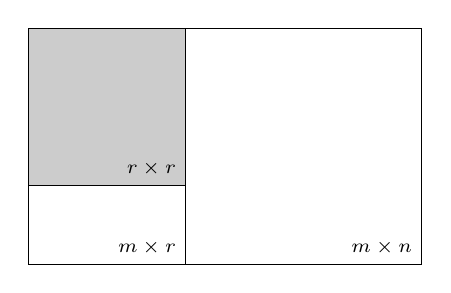
\begin{tikzpicture}
		\draw (0,0) rectangle (5,-3) node[above left]{\scriptsize $m \times n$};
		\draw (0,0) rectangle (2,-3) node[above left]{\scriptsize $m \times r$};
		\filldraw[fill=black!20!white] (0,0) rectangle (2,-2) node[above left]{\scriptsize $r \times r$};
	\end{tikzpicture}
	\end{center}

	\emph{(i) $\Rightarrow$ (ii)}: sei (i) erfüllt. Um (ii) herzuleiten, können wir im Wesentlichen unseren Beweis von (ii) $\Rightarrow$ (i) umkehren. Die Spalten von $A$ spannen einen Raum der Dimension mindestens $r$ auf. Wir können aus den Spalten von $A$ eine Basis des Spaltenraums auswählen. Diese Basis hat mindestens $r$ Vektoren, beliebige $r$ Vektoren aus der Basis, spannen einen $r$-dimensional Vektorraum auf. Da wir die Spalten beliebig vertauschen können, können wir ohne Beschränkung der Allgemeinheit annehmen, dass die ersten $r$ Spalten von $A$ solche $r$ linear unabhängige Vektoren sind. Das bedeutet, die $m \times r$ Untermatrix
	\[
		(a_{ij})_{i=1,\ldots,m, \ j=1,\ldots,r}
	\]
	hat den Rang $r$. Die Zeilen dieser Matrix spannen somit den $r$-dimesionalen Vektorraum  $\K^r$ auf. Man findet also unter den Zeilen der vorigen $m \times r$ Untermatrix eine Basis von $\K^r$. Da wir Zeilen von $A$ beliebig vertauschen können, können wir annehmen, dass die ersten $r$ Zeilen der vorigen $m \times r$ Untermatrix eine Basis von $\K^r$ bilden. Das bedeutet, dass die $r \times r$ Untermatrix 
	\[
		(a_{ij})_{i=1,\ldots,r, \ j=1,\ldots,r}
	\]
	den Rang $r$ hat. Daraus folgt, dass die Determinante dieser $r \times r$ Untermatrix ungleich $0$ ist. Somit ist (ii) erfüllt. 
\end{proof}

\begin{bsp}
	Die Intuition hinter dem vorigen Theorem wird aus der folgenden Beschreibung klar. Betrachten wir eine Nadel und eine Scheibe im dreidimensionalen Raum. Die Nadel ist eindimensional und die Scheibe ist zweidimensional. Nun wird die Nadel und die Scheibe von vorne, von oben und von der Seite fotografiert. Für die beiden Objekte kriegen wir je drei Fotos und müssen nun die Nadel von der Scheibe auseinanderhalten. Ein oder zwei Fotos reichen im Allgemeinen nicht aus. Wenn z.B. die Scheibe horizontal platziert ist, so sieht man an den Fotos von der Seite und von vorne die zweite Dimension nicht. Mit anderen Worten ist eine entsprechende Projektion der Scheibe eindimensional, obwohl die Scheibe zweidimensional ist. Da wir aber drei Fotos aus drei zueinander senkrechten Richtungen machen, sehen wir an mindestens einem der drei Fotos, dass die Scheibe mindestens zwei Dimensionen hat. Auf diese Weise lässt sich eine Scheibe von einer Nadel unterscheiden. 
	
	Was hier informell beschrieben ist ist eine Anwendung des vorigen Theorems im Fall $r=2$. Wir können die Anwendung aber auch rein formal illustrieren. Betrachten wir eine beliebige $3 \times 2$ Matrix
	\[
		A = \begin{pmatrix} a_{11} & a_{12} \\ a_{21} & a_{22} \\ a_{31} & a_{32} \end{pmatrix}.
	\]
	Der Rang von $A$ ist $0$, $1$ oder $2$. Wie können wir die Matrizen mit dem Rang höchstens $1$ und die Matrizen mit dem Rang $2$ auseinander halten? Die geometrische Interpretation ist die Folgende. Der Nullvektor $0$ und die beiden Spalten $a_1, a_2$ von $A$ bilden im nichtentarteten Fall die Ecken eines Dreiecks. Im entarteten Fall kann sich das Dreieck zu einer Strecke (Rang $1$) oder sogar zu einem Punkt (Rang $0$) entarten. Laut dem vorigen Theorem hat $A$ genau dann Rang $2$, wenn mindestens einer der drei $2 \times 2$ Minoren
	\begin{align*}
			M_1 & = \begin{vmatrix} a_{21} & a_{22} \\ a_{31} & a_{32} \end{vmatrix}, &
			M_2 & = \begin{vmatrix} a_{11} & a_{12} \\ a_{31} & a_{32} \end{vmatrix}, &
			 M_3 & = \begin{vmatrix} a_{11} & a_{12} \\ a_{21} & a_{22} \end{vmatrix}  
	\end{align*}
	ungleich $0$ ist. Mit anderen Worten hat $A$ genau dann den Rang höchstens $1$, wenn $M_1 = M_2 = M_3=0$ erfüllt ist (alle drei $2 \times 2$ Minoren gleich $0$). Wenn die Standardbasisvektoren $e_1$ nach vorne, $e_2$ zur Seite und $e_3$ nach oben gerichtet sind, dann entspricht der Minor $M_1$ dem Foto von vorne, $M_2$ dem Foto von der Seite und $M_3$ dem Foto von oben. Man kann nämlich sehen, dass $\frac{1}{2} M_i$ bis auf das Vorzeichen die Fläche des Schattens unseres Dreiecks bei der Projektion in Richtung $e_i$. Haben alle drei Projektion Fläche $0$, dann ist unser Dreieck entartet. 
\end{bsp}


\begin{bsp}
	Bei der Diskussion der Laplace-Entwicklung haben wir bereit einen durch zwei Vektoren aufgespannten zweidimensionalen Vektorraum in $\K^3$ (eine Ebene) eine Beschreibung durch eine Gleichung hergeleitet. Nun wollen wir eine durch ihre Richtung gegebene Gerade mit Gleichungen beschreiben. 
	
	Sei $ v \in \K^3 \setminus \{ 0 \} $. Wir beschreiben die Gerade $ \lin(v) $ durch lineare Gleichungen. Sei $ v = (a,b,c) $, $ a,b,c \in \K $.
	
	Der Vektor $ p = (x,y,z) \in \K^3 $ liegt genau dann auf der Geraden $\lin(v)$, wenn  die Vektoren $p$ und $v$ linear abhängig sind. Das ist genau dann der Fall, wenn der Rang der Matrix 
	\begin{equation*}
		\begin{pmatrix}
			x & a \\
			y & b \\
			z & c
		\end{pmatrix}
	\end{equation*}
	mit den Spalten $p$ und $v$ kleiner als zwei ist. Nach dem vorigen Theorem gilt das letztere genau dann, wenn alle $3$ Minoren unserer $3 \times 2$ Matrix gleich $0$ sind. 
	Das ergibt die Beschreibung von von $\lin(v)$ durch das System
	\[
		 \left\{ \begin{aligned}
		xb - ya &= 0 \\
		xc - za &= 0 \\
		yc - zb &= 0
	\end{aligned} \right. 
	\] 
	von $3$ linearen Gleichungen.  Intuitiv ist es klar, dass man eine Gerade im dreidimensionalen Raum durch nur zwei Gleichungen beschreiben kann. Eine der drei Gleichungen ist tatsächlich redundant, nur weiß man nicht genau welche, wenn man die Koordinaten $a,b,c$ des Richtungsvektors $v$ nicht genau spezifiziert, sonder allgemein hält. 
	
	Versuchen Sie z.B. im Fall von $\K=\R$ und $a=1, b=2, c=3$ eine Beschreibung der Geraden $\lin(v)$ mit nur zwei Gleichungen herzuleiten. Dabei können Ihnen ihre Kenntnisse über den Rang bestimmt helfen. 
\end{bsp}

\subsubsection{Der Satz von Binet-Cauchy}

Im Abschluss dieses Kapitels diskutieren wir einen weiteren allgemeinen Satz über die Determinanten, den sogenannten Satz von Binet-Cauchy. Für quadratische Matrizen $A$ und $B$ der gleichen Größe haben wir am Anfang des Kapitels die Formel $\det(A B) = \det(A) \det(B)$ hergeleitet. Wenn wir $B$ durch $B^\top$ austauschen und dann $\det(B^\top) = \det(B)$ benutzen, können wir die Formel auch als $\det(A B^\top) = \det(A) \det(B)$ formulieren. Es stellt sich heraus, dass für die vorige Formel eine Verallgemeinerung für nicht-quadratische Matrizen (gleicher Größe) existiert. Diese Verallgemeinerung ist der Gegenstand des Satzes von Cauchy-Binet. 

Die geometrische Interpretation des Satzes von Binet-Cauchy in einem Spezialfall  

\begin{thm}[Satz von Binet-Cauchy]
	Man betrachte $m \times n$ Matrizen $ A = (a_1, \ldots, a_n), B = (b_1, \ldots, b_n) \in \K^{m \times n} $ mit $ m \leq n $. Dann erfüllt die Determinante der $m \times m$ Matrix $A B^\top$ die Gleichung. 
	\begin{equation}
		\det(AB^\top) = \sum_{1 \leq i_1 < \ldots < i_m \leq n} \det(a_{i_1}, \ldots, a_{i_m}) \det(b_{i_1}, \ldots, b_{i_m}).
	\end{equation}
	(Die Summe geht über alle $i_1,\ldots,i_m \in \{1,\ldots,n\}$ mit $1 \le i_1 < \cdots < i_m \le n$ und hat somit $\binom{n}{m}$ Summanden). 
\end{thm}

Im Satz von Binet-Cauchy wird die Determinante von $A B^\top$ mit der Verwendung aller $m \times m$ Minoren von $A$ und $B$ dargestellt.  Die jeweiligen Minoren von $A$ und $B$ werden miteinander multipliziert, und alle solche Produkte von Minoren werden zusammengerechnet. 


\begin{proof}[Beweis des Theorems]
	Wir leiten die Formel mit der Verwendung der Grundeigenschaften der Determinante (die Determinante ist linear in jeder Spalte und alternierend bzgl. der Spalten). Die Spalten von $A B^\top$ sind Linearkombinationen der Spalten von $A$. Dh., wenn wir die Komponenten von $B$ als $b_{ij}$ bezeichnen, so erhalten wir 
	\begin{align*}
		AB^\top &= \begin{pmatrix}
			| && | \\
			a_1 & \cdots & a_n \\
			| && |
		\end{pmatrix} \begin{pmatrix}
			b_{11} & \cdots & b_{m1} \\
			\vdots &  & \vdots \\
			b_{1n} & \cdots & b_{mn}
		\end{pmatrix} \\
		&= \begin{pmatrix}
			| && | \\
			\sum_{j=1}^n a_jb_{1j} & \cdots & \sum_{j=1}^n a_jb_{mj} \\
			| && |
		\end{pmatrix}		
	\end{align*}
	D.h. für $ k \in \is{1}{m} $ hat die $ k $-te Spalte von $ AB^\top $ die Form $ a_1b_{k1} + \ldots + a_nb_{kn} = \sum_{j=1}^{n} a_jb_{kj} $. Jeder der $m$ Spalten von $A B^\top$ also also Linearkombination von jeweils $n$ Vektoren. Eine Linearkombination ist eine Summe, und wir wollen nun all diese $m$ Summen als eine `große Summe'  zusammenfassen. Wir erhaltne mit der Verwendung der Linearität in den Spalten die Gleichung: 
	\begin{align*}
		\det(AB^\top) &= \det\left( \sum_{j_1=1}^{n} a_{j_1}b_{1,j_1}, \ldots, \sum_{j_m=1}^{n} a_{j_m}b_{m,j_m} \right) \\
		&= \sum_{j_1, \ldots, j_m \in \is{1}{n}} \det(a_{j_1}, \ldots, a_{j_m}) \cdot b_{1,j_1} \cdots b_{m,j_m}.
	\end{align*}
	Die vorige Summe der $m^n$ Summanden hat viele Nullen. 
	Das die Determinante alternierendes Funktional ist gilt: Wenn mindestens 2 der Werte $ j_1, \ldots, j_m $ gleich sind, ist $ \det(a_{j_1}, \ldots, a_{j_m}) = 0 $. Daher kann man sich in der vorigen Summe auf $ j_1, \ldots, j_m \in \is{1}{m} $ beschränken, deren Werte paarweise verschieden sind. In diesem Fall kann die $ m $-elemtige Menge $ \is{j_1}{j_m} $ \textquote{aufsteigend nummeriert} werden, d.h. es existieren $ i_1, \ldots, i_m \in \is{1}{n} $ mit $ i_1 < \ldots < i_m $ und $ \is{j_1}{j_m} = \is{i_1}{i_m} $.
	
	Sei $ \sigma \in S_m $ eine Permutation mit $ j_1 = i_{\sigma(1)}, \ldots, j_m = i_{\sigma(m)} $. [Bspw. für $ j_1 = 3, j_2 = 1, j_3 = 7 $ sind $ i_1 = 1, i_2 = 3, i_3 = 7 $ und $ \sigma(1) = 2, \sigma(2) = 1, \sigma(3) = 3 $.] Die Permutation $ \sigma $ und die Indizes $ i_1, \ldots, i_m $ sind durch die Wahl von $ j_1, \ldots, j_m $ eindeutig bestimmt. Wir setzen für $ j_1 = i_{\sigma(1)}, \ldots, j_m = i_{\sigma(m)} $ ein und erhalten
	\begin{align*}
		\det(AB^\top) &= \sum_{\substack{\sigma \in S_m \\ 1 \leq i_1 < \ldots < i_m \leq n}} \det(a_{i_{\sigma(1)}}, \ldots, a_{i_{\sigma(m)}}) \cdot b_{1,i_{\sigma(1)}} \cdots b_{m,i_{\sigma(m)}} \\
		&= \sum_{\substack{\sigma \in S_m \\ 1 \leq i_1 < \ldots < i_m \leq n}} \det(a_{i_1}, \ldots, a_{i_m}) \sign(\sigma) \cdot b_{1,i_{\sigma(1)}} \cdots b_{m,i_{\sigma(m)}} \\
		&= \sum_{1 \leq i_1 < \ldots < i_m \leq n} \det(a_{i_1}, \ldots, a_{i_m})
		\underbrace{\sum_{\sigma \in S_m} \sign(\sigma) \cdot b_{1,i_{\sigma(1)}} \cdots b_{m,i_{\sigma(m)}}
		}_{\text{Leibnizformel für } (b_{i_1}, \ldots, b_{i_m})} \\
		&= \sum_{1 \leq i_1 < \ldots < i_m \leq n} \det(a_{i_1}, \ldots, a_{i_m}) \det(b_{i_1}, \ldots, b_{i_m}) \qedhere
	\end{align*}
\end{proof}

\begin{proof}[Ein anderer Beweis des Satzes von Binet-Cauchy]
	Wir bezeichnen als $A_{I,J}$ die Untermatrix zu den Zeilen bzw. Splaten, die durch $I$ bzw. $J$ indexiert sind. des Weiteren seien $[m] := \{1,\ldots,m\}$ und $[n] := \{1,\ldots, n\}$ und sei $\binom{[n]}{m}$ die Menge aller $m$-elementigen Teilmengen von $[n]$. Dann kann die Binet-Cauchy-Formel als 
	\[
		\det(A B^\top) = \sum_{I \in \binom{[n]}{m}} \det(A_{[m], I }) \det(B_{[m], I}) 
	\]
	formuliert werden. Wir können $A B^\top$ mit Hilfe der Zeilen $B_{1,[n]},\ldots, B_{m,[n]}$ von $B$ wie folgt darstellen: 
	\[
		 ( A B_{1,[n]}^\top,\ldots, A B_{m,[n]}^\top) . 
	\]
	Da die Determinante linear in den Spalten ist zeigt das, dass 
	\[
		\det(A B^\top) = \det( A B_{1,[n]}^\top,\ldots, A B_{m,[n]}^\top) 
	\]
	als Funktion der Spalten von $B$ in jeder der $m$ Zeilen von $B$ linear  ist. Des Weiteren ist die Funktion alternierend in der Zeilen von $B$, weil die Determinante alternierend ist. 
	
	 Das Gleiche gilt für die rechte Seite der Formel, die wir beweisen,  die rechte Seite ist linear in den Zeilen von $B$ und alternierend, denn 
	\[
	\sum_{I \in \binom{[n]}{m}} \det(A_{[m], I }) \det(B_{[m], I})  = \sum_{I \in \binom{[n]}{m}} \det(A_{[m], I }) \det(B_{1, I}, \ldots, B_{m,I}). 
	\]
	Aus der multlinearität in den Zeilen von $B$ folgt, dass die Formel im allgemeinen Fall gilt, sobald wir sie im Fall verifizeiren, bei dem $B$ Vektoren aus der Standardbasis von $\K^n$ sind: also für	 $B_{1,[n]},\ldots,B_{m,[n]} \in \{e_1^\top,\ldots, e_n^\top\}$. 	Sei also 
	$B_{i,[n]} = e_{k_i}^\top$ mit $k_1,\ldots,k_m \in [n]$. Da die beiden Seiten alternierend sind, kriegen wir auf der linken und rechte Seite eine $0$, wenn $B$ zwei identische Zeilen hat. Wir können also annehmen, dass $k_1,\ldots, k_m$ paarweise verschieden sind. Da die linken und die rechten Seiten alternierend sind, verursacht das vertauschen von zwei Zeilen von $B$ eine Vorzeichenänderung auf beiden Seiten. Wir können also durch das Vertauschen der Zeilen, die Formel auf den Fall $k_1 < \cdots < k_m$ zurückführen. Nach diesen Veränderungen ist die linke Seite 
	\begin{align*}
		\det (A B^\top) & = \det (A B_{1,[n]}^\top \cdots A B_{m,[n]}^\top) 
		\\ & = \det ( A ( e_{k_1} \cdots e_{k_m} ) 
		\\ &  = \det (A e_{k_1},\ldots, A e_{k_m}) 
		\\ & = \det(A_{[m], \{k_1,\ldots,k_m\}}). 
	\end{align*} 
	Die rechte Seite ist 
	\begin{align*} 
		\sum_{I \in \binom{[n]}{m}} \det(A_{[m], I }) \det(B_{1, I}, \ldots, B_{m,I}) = \sum_{I \in \binom{[n]}{m}} \det(A_{[m], I }) \det( (e_{k_1} \cdots e_{k_m})_{I,[m]} ), 
	\end{align*}
	wobei die Matrix $ (e_{k_1} \cdots e_{k_m})_I $ im Fall $I \ne \{k_1,\ldots,k_m\}$ die Determinante $0$ hat, weil dann ein Element $i \in I \setminus \{k_1,\ldots,k_m\}$ existiert, woraus folgt, dass die genannte Matrix eine Nullzeile besitzt. Auf der rechten Seite bleibt also nur der Term für $I= \{k_1,\ldots,k_m\}$, un dieser Term ist gleich $\det(A_{[m], \{k_1,\ldots,k_m\}}). $
\end{proof} 


\begin{bem} Besonders interessant ist der Fall $A =B$ des Satzes Binet-Cauchy. In diesem Fall ist die rechte Seite der Formel die Summe der Quadrate aller $m \times m$ Minoren von $A$. Wenn unser Körper der Körper der reellen Zahlen ist, wissen wir also, dass $\det(A A^\top)$ ein nicht-negativer Wert ist. Wir können also die Wurzel ziehen und kommen zur Gleichung
	\begin{equation*}
		\sqrt{\det(AA^\top)} = \sqrt{\sum_{1 \leq i_1 < \ldots < i_m \leq n} \det(a_{i_1}, \ldots, a_{i_m})^2}.
	\end{equation*}
	Die vorige Gleichung hat eine Geometrische Bedeutung. Sie ist im gewissen Sinne eine weitreichende Verallgemeinerung des Satzes von Pythagoras, über den Sie in der Schule gehört haben könnten. 


	Sind $z_1,\ldots,z_m$ die Zeilen von $A$, dann ist der Wert
	$ \sqrt{\det(AA^\top)} $ das $ m $-dimensionale Volumen des sogenannten  Hyperparallelepipeds $ [0,1]z_1 + \ldots + [0,1]z_m = \{ \sum_{i=1}^m \alpha_iz_i : \alpha_i, \ldots, \alpha_m \in [0,1] \} $,
	das durch die Vektoren $z_1,\ldots,z_m$ aufgespannt ist. Die Formel von Binet-Cauchy beschreibt das Volumen des $m$-dimensionalen Hyperparallelepipeds in der Dimension $n$ durch die Volumina seiner `Schatten'  beim Projizieren auf $m$-dimensionale Räume, welche durch die Standardbasisvektoren aufgespannt sind. 
	
	Am einfachsten lässt sich der Fall von Parallelogrammen in der Dimension drei veranschaulichen. Wir sehen die Photos einer Scheibe von vorne, von der Seite und von oben, messen die Flächen der Bilder der Scheibe auf allen drei Fotos und wollen anhand dieser Flächen die Fläche der Scheibe ausrechnen. Das geht tatsächlich: die Fläche der Scheibe ist die Wurzel aus der Summe der Quadraten der Flächen der Bilder. 
\end{bem}

\begin{bsp}
	Berechnen wir die Fläche des Dreiecks mit Ecken $(0,0,0)$, $(2,7,5)$ und $(8,1,4)$ ist mit der Verwendung der linken Seite der Binet-Cauchy-Formel.
	
	\begin{center}
	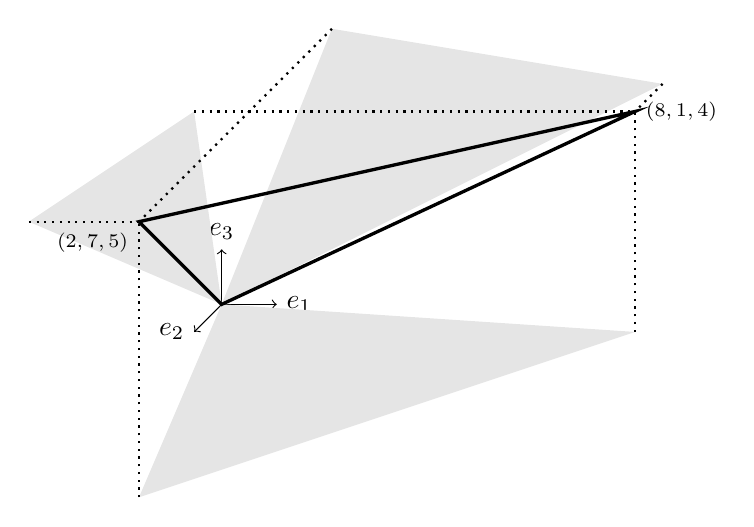
\begin{tikzpicture}[scale=0.7]
		\def\ax{2}
		\def\ay{7}
		\def\az{5}
		%
		\def\bx{8}
		\def\by{1}
		\def\bz{4}
		%
		\draw[->] (0,0) -- (1,0) node[right]{$e_1$};
		\draw[->] (0,0) -- (0,1) node[above]{$e_3$};
		\draw[->] (0,0) -- (-0.5,-0.5) node[left]{$e_2$};
		%
		\fill[black!10!white] (0,0) -- ({-0.5*\ay},{\az-0.5*\ay})  -- ({-0.5*\by},{\bz-0.5*\by})-- cycle;
		\fill[black!10!white] (0,0) -- ({\ax},{\az})  -- ({\bx},{\bz})  -- cycle;
		\fill[black!10!white] (0,0) -- ({\ax-0.5*\ay},{-0.5*\ay})  -- ({\bx-0.5*\by},{-0.5*\by}) -- cycle;
		%
		\draw[very thick] (0,0) -- ({\ax-0.5*\ay},{\az-0.5*\ay}) node[below left]{\scriptsize $(2,7,5)$} -- ({\bx-0.5*\by},{\bz-0.5*\by}) node[right]{\scriptsize $(8,1,4)$} -- cycle;
		%
		\draw[dotted,thick] ({-0.5*\ay},{\az-0.5*\ay}) -- ({\ax-0.5*\ay},{\az-0.5*\ay});
		\draw[dotted, thick] ({\ax},{\az}) -- ({\ax-0.5*\ay},{\az-0.5*\ay});
		\draw[dotted, thick] ({\ax-0.5*\ay},{-0.5*\ay}) -- ({\ax-0.5*\ay},{\az-0.5*\ay});
		%
		\draw[dotted,thick] ({-0.5*\by},{\bz-0.5*\by}) -- ({\bx-0.5*\by},{\bz-0.5*\by});
		\draw[dotted, thick] ({\bx},{\bz}) -- ({\bx-0.5*\by},{\bz-0.5*\by});
		\draw[dotted, thick] ({\bx-0.5*\by},{-0.5*\by}) -- ({\bx-0.5*\by},{\bz-0.5*\by});
	\end{tikzpicture}
	\end{center}
	Die Projektionen auf die drei Koordinatenebenen sind die drei Dreiecke: 
	\begin{itemize}
		\item In Richtung $e_1$: Dreieck $T_1$ mit den Ecken $(0,0), (7,5)$ und $(1,4)$,
		\item In Richtung $e_2$: Dreieck $T_2$ mit den Ecken $(0,0), (2,5)$ und $(8,4)$,
		\item In Richtung $e_3$: Dreieck $T_3$ mit den Ecken $(0,0), (2,7)$ und $(8,1)$. 
	\end{itemize} 
	Die Flächen der drei Dreiecken ergeben sich aus den drei $2 \times 2$ Minoren der Matrix 
	\begin{equation*}
		A= 
			\begin{pmatrix} 
				2 & 7 & 5
				\\ 1 & 8 & 4
			\end{pmatrix} 
	\end{equation*}
	Die drei Minoren sind 
	\begin{align*}
			\begin{vmatrix} 
				 7 & 5
				 \\ 8 & 4
			\end{vmatrix} 
			& = -12, 
			& 
			\begin{vmatrix} 
			2 & 5
		\\ 1 & 4
		\end{vmatrix} 
			&	 = 3, 
			&
			\begin{vmatrix} 
	2 & 7
	\\ 1 & 8
\end{vmatrix} 
&	 = 9.
	\end{align*}
	Die Fläche von $T_1$, $T_2$ und $T_3$ ist somit jeweils $6$, $\frac{3}{2}$ und $\frac{9}{2}$. Die Fläche von unserem Dreieck in der Dimension drei ist somit 
	\[
		\sqrt{ 6^2 + \left( \frac{3}{2} \right)^2 + \left( \frac{9}{2} \right)^{2}} = \sqrt{58{,}5}.
	\]
	Man kommt auf den selben Wert, wenn man die Fläche unseres Dreiecks mit Hilfe der linken Seite der Binet-Cauchy-Formel als $\frac{1}{2} \sqrt{\det(A A^\top)}$ berechnet. (Die Berechnung durch die Fläche der drei Projektion haben wir hier zur Veranschaulichung der Binet-Cauchy-Formel gegeben. Es ist keine Empfehlung: man muss die Fläche nicht unbedingt auf diese Weise berechnen, die Verwendung von $\sqrt{\det(A A^\top)}$ führt einen schneller zum Ziel.) 
\end{bsp}

\subsubsection{Die Formel von Sylvester} 

\begin{thm}
	Seien $A \in \K^{m \times n}$ und $B \in \K^{n \times m}$. Dann gilt $\det(I_m + A B) = \det(I_n + B A)$. 
\end{thm} 
\begin{proof} 
	Es gilt 
	\begin{align*}
			\begin{pmatrix} I_m & 0 \\ B & I_n \end{pmatrix} \begin{pmatrix} I_m & 0 \\ 0 & I_n - B A  \end{pmatrix}  \begin{pmatrix} I_m & A \\ 0 & I_n \end{pmatrix} & = \begin{pmatrix} I_m & A \\ B & I_n \end{pmatrix} \\ & = \begin{pmatrix} I_m & 0 \\ B & I_n \end{pmatrix} \begin{pmatrix} I_m - A B  & 0 \\ 0 & I_n   \end{pmatrix}  \begin{pmatrix} I_m & A \\ 0 & I_n \end{pmatrix}
	\end{align*}
Durch die Anwendung von $\det$ zu dieser Gleichung erhalten wir die gewünschte Gleichung. 
\end{proof} 
